% Paper 1: Knowledge Graph Quality Assessment and Enhancement
% Focus: Innovation 1 (Quality Aggregation Model) + Innovation 3 (Multi-dimensional Analysis Framework)

\documentclass[pdflatex,sn-basic]{sn-jnl}

% \documentclass[runningheads]{llncs}
\usepackage{graphicx}
\usepackage{amsmath,amssymb,amsfonts}
\usepackage{bbm} % for \mathbbm{1} indicator function
\usepackage{amsthm}
\usepackage{mathrsfs}
% \usepackage[title]{appendix} % removed (no appendix section in the paper)

\usepackage{tabularx}
\usepackage{xcolor}
% \usepackage{textcomp}
\usepackage{booktabs}
% \usepackage{multirow}
% \usepackage{makecell}

\usepackage{pgfplots}
\usepackage{tikz}
\pgfplotsset{compat=1.18}
\usepackage{pgfplotstable}
\pgfplotsset{
    every axis/.append style={
        width=\textwidth,
        height=7cm,
        grid=major,
        grid style={dashed,gray!30},
        legend pos=north west,
        legend style={font=\footnotesize},
        label style={font=\footnotesize},
        tick label style={font=\footnotesize},
        axis lines=left,
        enlarge x limits=0.1,
    }
}
\usepackage{algorithm}
\usepackage{algpseudocode}

\usepackage{fontspec}
\setmainfont{Noto Serif CJK SC}[SmallCapsFont={Noto Serif CJK SC},ItalicFont={Noto Serif CJK SC},ItalicFeatures={FakeSlant=0.15},BoldItalicFont={Noto Serif CJK SC Bold},BoldItalicFeatures={FakeSlant=0.15}]
\setsansfont{Noto Sans CJK SC}
\setmonofont{Noto Sans Mono CJK SC}[Scale=0.85]
\XeTeXlinebreaklocale "zh"
\XeTeXlinebreakskip=0pt plus 1pt
\setlength{\emergencystretch}{3em}
\setlength{\bibsep}{0.7em}
\renewcommand{\figurename}{图}
\renewcommand{\tablename}{表}
\renewcommand{\refname}{参考文献}
\renewcommand{\appendixname}{附录}
\renewcommand{\abstractname}{摘要}
\def\keywordname{关键词}
\floatname{algorithm}{算法}
\algrenewcommand{\algorithmicrequire}{输入：}
\algrenewcommand{\algorithmicensure}{输出：}
\algrenewcommand{\algorithmicfor}{对}
\algrenewcommand{\algorithmicdo}{执行}
\algrenewcommand{\algorithmicif}{若}
\algrenewcommand{\algorithmicthen}{则}
\algrenewcommand{\algorithmicelse}{否则}
\algrenewcommand{\algorithmicend}{结束}
\algrenewcommand{\algorithmicreturn}{返回}


\graphicspath{{figure/}}

%% as per the requirement new theorem styles can be included as shown below
\theoremstyle{thmstyleone}%
\newtheorem{theorem}{Theorem}%  meant for continuous numbers
%%\newtheorem{theorem}{Theorem}[section]% meant for sectionwise numbers
%% optional argument [theorem] produces theorem numbering sequence instead of independent numbers for Proposition
\newtheorem{proposition}[theorem]{Proposition}% 
%%\newtheorem{proposition}{Proposition}% to get separate numbers for theorem and proposition etc.
\theoremstyle{thmstyletwo}%
\newtheorem{example}{Example}%
\newtheorem{remark}{Remark}%
\theoremstyle{thmstylethree}%
\newtheorem{definition}{Definition}%

\raggedbottom
%%\unnumbered% uncomment this for unnumbered level heads

\begin{document}

\title{利用源文本与字段检查修复文档知识图谱}

% \titlerunning{Constraint-Based KG Quality Enhancement}

%%=============================================================%%
%% GivenName	-> \fnm{Joergen W.}
%% Particle	-> \spfx{van der} -> surname prefix
%% FamilyName	-> \sur{Ploeg}
%% Suffix	-> \sfx{IV}
%% \author*[1,2]{\fnm{Joergen W.} \spfx{van der} \sur{Ploeg} 
%%  \sfx{IV}}\email{iauthor@gmail.com}
%%=============================================================%%

\author[1]{\fnm{Hua} \sur{Peng}}\email{penghua@cmict.chinamobile.com}
\equalcont{以上作者对本文贡献相同。}

\author[2]{\fnm{Zifu} \sur{Tao}}\email{2253323@tongji.edu.cn}
\equalcont{以上作者对本文贡献相同。}

\author[1]{\fnm{Yu} \sur{Guo}}\email{guoyu1@cmict.chinamobile.com}

\author[2]{\fnm{Qiang} \sur{Zhou}}\email{zhouqiang@cmict.chinamobile.com}

\author*[3]{\fnm{Tian} \sur{Zhou}}\email{tianzhou@xjtu.edu.cn}

\author[3]{\fnm{Bo} \sur{Han}}\email{bohan@xjtu.edu.cn}

\affil[1]{\orgname{中移系统集成有限公司}, \country{中国}}

\affil[2]{\orgname{同济大学}, \country{中国}}

\affil[3]{\orgname{西安交通大学}, \country{中国}}

% \affil[1]{\orgdiv{Department}, \orgname{Organization}, \orgaddress{\street{Street}, \city{City}, \postcode{10587}, \state{State}, \country{Country}}}

% Springer front matter must be defined before \maketitle.
\abstract{
从文档构建的知识图谱可能有字段缺失和取值错误。我们利用源文本和字段规则，将图检查与修复结合。局部、图和来源检查组成评估概况。主路径先清理输入，再让语言模型生成图，最后按字段约束过滤三元组。我们还测试尺度感知路由，每次为一个候选编辑赋予权重并进行检查。共享提示和过滤前后的评分展示各步骤的变化。在包含 450 个注入缺陷的 225 张图上，诊断＋门控 修复了 98.00\% 的缺陷。在 225 张模型构建图上，三元组 F1 从 87.99\% 提高到 92.48\%。直接字段复制在这些记录上达到 100\%。在 60 张新收据的测试中，来源行索引使 F1 比 简单流程 高 4.76 个百分点（95\% 置信区间：2.50 至 7.26）。在 56 份 CUAD 合同上，索引修复的 F1 为 44.84\%，输入为 46.76\%；与索引重新抽取的 F1 差为 0.72 个百分点（95\% 置信区间：$-4.80$ 至 6.48）。两名评审检查 200 项参考差异和 200 项系统编辑，在 200 项差异中的 95 项发现输入错误。第三名评审解决分歧后，五种设置中的 199 项确定编辑有 134 项被接受，另有一项仍不确定。实验展示源文本、字段检查和输入图如何影响修复。代码、模型输出和评价规则已提供，供后续研究使用。
}
\keywords{知识图谱修复，源文本，字段检查，文档抽取}
\maketitle
\begin{center}\footnotesize 中文完整译本，对应英文合并版。参考文献保留原始出版信息；模型标识与程序名称保留原文。图内英文标注的中文对照见译文附页。\end{center}
% Introduction
\section{引言}
\label{sec:introduction}

知识图谱（KG）用三元组保存事实。每条三元组包含主体、关系和值。例如，收据图谱可以保存收据编号、字段“total”和取值“120.00”。从文本构建的图谱常有值缺失、值错误、三元组重复或关系不合法等问题\citep{ref_ji2021,ref_paulheim2017}。修复需要先找到这些错误，再选择与原文相符的修改。

第一个问题是决定检查什么。三元组重复、字段不合法和值错误的原因各不相同。质量检查工具覆盖结构、规则和事实内容\citep{ref_zaveri2016,ref_kontokostas2014,ref_wang2021}。我们按实体、图和上下文三个范围组织检查。它们查找重复事实，检查文档编号和字段名，并将取值与原文匹配。这些结果共同组成评估概况，记录哪些位置需要修复。

第二个问题是决定保留哪些修改建议。模型可以阅读文本并提出取值，但每个字段也有相应规则。SHACL 用于表达图规则，近期修复方法将这些规则加入大语言模型提示\citep{ref_shacl2017,ref_lin2025}。我们用来源和字段约束检查生成的三元组。过滤器在允许的关系和字段数量范围内，保留与来源匹配的值，并记录每条被拒绝三元组的原因。

第三个问题是在修复动作中作出选择。多个建议可能针对同一字段，一次编辑也可能影响其他检查。规则、学习模型和源文本提供了不同的图修复方式\citep{ref_paulheim2017,ref_pan2023}。我们测试尺度感知路由，用评估概况为各类编辑赋予权重。选择器在图副本上试改候选，检查边界，并为每项编辑打分。它执行得分最高且为正的允许编辑，然后再次检查图。

本文任务使用保存单篇文档字段的图。每张图具有固定文档编号和允许关系名单。每种关系最多对应一个值。主修复路径先清理输入，再根据原文生成完整图，最后过滤其中的三元组。错误报告或来源行提示可以引导模型。我们分别为这条路径和顺序选择器设置对照，并保存各自的执行日志。

实验使用三个中文记录集合、SROIE 收据和 CUAD 合同。我们用 20 张新收据设置来源行索引，然后冻结设计，在另外 60 张收据上测试。合同测试使用 56 份文档。两名评审检查 200 项参考差异和 200 项系统编辑。共享提示以及同一输出过滤前后的评分展示各步骤的作用。实验衡量字段恢复、事实保留、请求成本和人工编辑接受度。

本文有三项贡献：
\begin{itemize}
    \item 将局部、图和来源检查汇入评估概况，在字段约束下引导基于来源的修复。
    \item 设计输出过滤流程，并单独测试尺度感知选择器，比较试改收益、成本和图边界。
    \item 在注入缺陷、模型输出、收据和合同上比较组件，开展人工评价，并公开输出和决策日志。
\end{itemize}

第~\ref{sec:related_work}~节回顾相关工作。第~\ref{sec:framework}、\ref{sec:implementation}~节介绍方法与实现。第~\ref{sec:experiments}~节报告实验和结果。第~\ref{sec:conclusion}~节总结全文。


% Related Work
\section{相关工作}
\label{sec:related_work}

\subsection{图构建与抽取事实检查}

构建知识图谱包括抽取事实、链接实体、映射关系和合并结果\citep{ref_ji2021}。DBpedia\citep{ref_auer2007}、YAGO\citep{ref_suchanek2007} 和 Freebase\citep{ref_bollacker2008} 从具有明确或部分明确结构的数据中建立知识库。知识融合利用来源证据为事实打分\citep{ref_dong2014}。这些检查帮助抽取过程选择事实。本文研究抽取后的图修复，并用原文检查取值。

嵌入模型用向量预测链接\citep{ref_bordes2013,ref_wang2017}。图神经网络从邻近节点和关系中学习\citep{ref_schlichtkrull2018}。相关综述介绍了利用大语言模型构建、补全和整合知识图谱的方法\citep{ref_pan2023,ref_pan2025,ref_bian2025}。提示方法包括思维链推理\citep{ref_wei2023}和共享提示模式\citep{ref_white2023}。检索增强生成将来源证据加入模型输入\citep{ref_lewis2020}。Neo4j Labs 的 LLM Knowledge Graph Builder 按用户设置的模式，将文档转换成图\citep{ref_neo4j_llm_graph_builder}。第~\ref{sec:eval:external_benchmark}~节将本文方法与其核心抽取器比较。

\subsection{图质量与检查范围}

知识图谱质量涉及事实正确、事实缺失、规则一致和信息时效\citep{ref_zaveri2016,ref_paulheim2017}。统计方法查找异常值\citep{ref_wienand2014,ref_paulheim2014}。嵌入模型为三元组的可信程度打分\citep{ref_nickel2016}。规则语言检查图的模式\citep{ref_kontokostas2014}。这些方法各自检查图质量的一部分。局部检查查找重复事实和无连接节点。图规则检查类型与关系。来源检查将记录值与文档证据匹配。评估概况将这些结果汇总，供修复过程共同使用。

Lin 等人向图中加入规则错误，并比较大语言模型修复提示\citep{ref_lin2025}。他们使用 SHACL 规则和邻近图上下文。人工评价有助于判断答案不明确的情况\citep{ref_acosta2013}。其他综述讨论图构建与修复中的质量检查\citep{ref_wang2021,ref_paulheim2017}。本文错误报告列出重复三元组、模式错误，以及未在原文中出现的值。

\subsection{图修复与动作选择}

知识图谱补全预测缺失链接。相关方法使用路径\citep{ref_lao2011}、嵌入\citep{ref_bordes2013,ref_yang2015,ref_shi2017}和神经网络\citep{ref_dettmers2018}。MINERVA 学习沿图路径回答查询\citep{ref_das2018}。MetaR 根据少量样本预测链接\citep{ref_chen2019}。AMIE 学习正规则\citep{ref_galarraga2013}，RuDiK 学习正规则和负规则\citep{ref_ortona2018}。其他方法将规则加入嵌入训练\citep{ref_guo2016,ref_ding2018}。

RNNLogic 联合训练规则生成器和答案预测器\citep{ref_qu2021}。NBFNet 从图路径中学习以预测链接\citep{ref_zhu2021}。pLogicNet 结合逻辑规则和嵌入\citep{ref_qu2019}。这些方法将规则与学习得到的预测结合。本文将源文本与字段检查结合。主路径过滤生成的图。尺度感知选择器根据评估概况为候选编辑赋予权重，并在图边界约束下比较试改分数。

Lin 等人比较了基于 SHACL 的修复提示\citep{ref_lin2025}。ReAct 将模型推理与信息收集动作结合\citep{ref_yao2023react}。本文的 ReAct-style 基线使用这一模式。我们的 SHACL 上下文基线将 Lin 等人的五部分提示改编到相同字段任务和调用上限下。共享提示以及过滤前后的评分展示上下文与图检查的作用。

% Methodology: problem formulation and implementation
\section{任务与方法}
\label{sec:framework}
\label{sec:framework:problem}

图修复需要两个相连的步骤：找到问题，再选择修改。我们连接图检查模块与修复模块。检查模块根据图和源文本构建评估概况。修复模块利用这一概况提出修改，并检查输出。

输入包括三元组列表 $G$、源文本 $X$、固定文档编号 $h_0$ 和允许关系 $\mathcal R_X$。列表可以包含同一三元组的多个副本。每种关系最多对应一个非空值，例如文档字段和收据字段。评分器用参考图 $G^*$ 检查输出。修复后的图记为 $\widehat G$。

主修复路径先清理输入，再让模型生成完整图，最后过滤三元组。错误报告或来源行提示可以引导生成。过滤器根据源文本和字段规则检查每个值。第二条路径利用尺度感知路由，每次选择一项编辑。它为试改后的图打分，并执行最佳允许编辑。第~\ref{sec:implementation}~节介绍两条路径及其测试设置。

\subsection{输入清理与错误报告}
\label{sec:framework:profile}

不同错误需要不同检查。重复三元组属于局部错误。错误的文档编号或字段名违反图规则。未在来源中出现的值无法通过证据检查。我们按实体、图和上下文三个范围组织检查。这里的上下文指文档源文本。图~\ref{fig:scale_relationship}~展示这三类检查。

\begin{figure}[t]
    \centering
    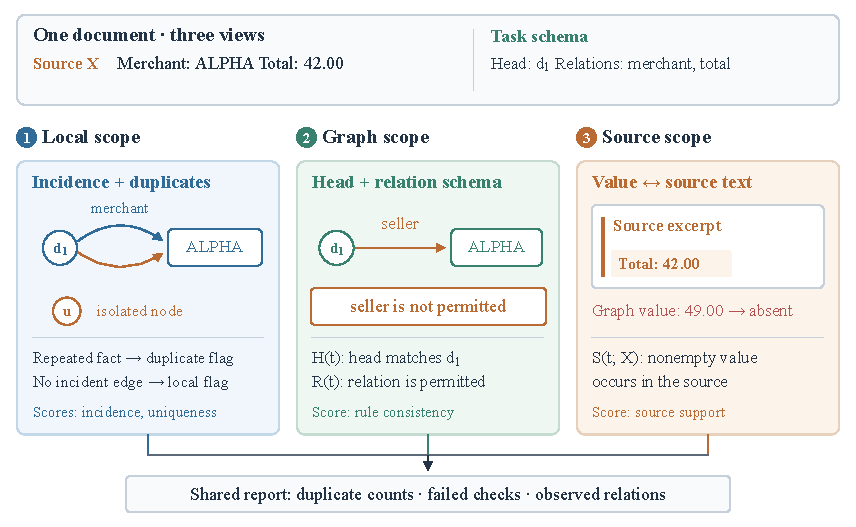
\includegraphics[width=0.98\textwidth]{figure/method/image2.pdf}
    \caption{图检查的三个范围。局部检查查找重复事实和无连接节点，图检查测试文档编号和字段名，来源检查在文本中查找值。两条修复路径都用这些检查构建评估概况。}
    \label{fig:scale_relationship}
\end{figure}

清理首先用明确的规则修正错误。预处理器 $P$ 删除重复三元组。若一条边的对象为 $h_0$，而主体是其他节点，则将该边反向。随后删除头节点或关系不合法的三元组。这里，头节点就是三元组的主体。清理后的图为 $G_s=P(G;h_0,\mathcal R_X)$。

对三元组 $t=(h,r,o)$，三项检查为
\begin{equation}
    \label{eq:diagnostic_predicates}
    H(t)=\mathbf1[h=h_0],\quad
    R(t)=\mathbf1[r\in\mathcal R_X],\quad
    S(t;X)=\mathbf1[o\ne\emptyset\ \wedge\ o\text{ 出现在 }X].
\end{equation}
$H$ 检查文档编号，$R$ 检查关系，$S$ 检查来源。分开执行这些检查，可以说明每条三元组被拒绝的原因。

主路径以错误报告的形式保存评估概况：
\begin{equation}
    \label{eq:diagnostic_context}
    D(G_s,X)=\big(n_{\mathrm{dup}},I_H,I_R,I_S,\mathcal R(G_s)\big).
\end{equation}
报告记录重复数、未通过检查的位置和已出现的关系。例如，$I_S=\{i:S(t_i;X)=0\}$ 列出未通过来源检查的位置。报告基于清理后的输入构建。它为模型提出字段值时提供查找位置。我们测试将报告加入提示的效果。字段为可选项，主路径对每篇文档调用模型一次。

\subsection{根据源文本生成图}
\label{sec:framework:architecture}

规则修正明确的结构错误；语言模型从文本中读取取值，并返回有序三元组列表：
\begin{equation}
    \label{eq:proposal_generation}
    C=L_\theta(X,h_0,\mathcal R_X,G_s,D(G_s,X)).
\end{equation}
提示要求模型生成完整图，复制来源值，保留正确字段，并补充或修正缺失、错误的值。JSON 解析器将无效响应记为空图。这些空图也计入评分。基础提示使用相同输入和输出上限，但去掉错误报告。

\subsection{检查生成的三元组}
\label{sec:framework:constraints}

约束决定哪些候选三元组进入修复后的图。门控是一个过滤器，在允许字段下保留与来源匹配的值，并保证每种关系最多有一个值。令 $\operatorname{uniq}(C)$ 按输出顺序去重。通过检查的三元组为
\begin{equation}
    \label{eq:eligible_candidates}
    C_X=\{t\in\operatorname{uniq}(C):H(t)R(t)S(t;X)=1\}.
\end{equation}
允许的输出集合为
\begin{equation}
    \label{eq:admissible_subsets}
    \mathcal F(C_X)=\left\{A\subseteq C_X:
    \sum_{t\in A}\mathbf1[r_t=r]\leq1,\ \forall r\in\mathcal R_X\right\}.
\end{equation}
式~\ref{eq:eligible_candidates}~规定证据和模式要求，式~\ref{eq:admissible_subsets}~规定字段数量上限。两者共同决定过滤器可以保留哪些输出。

过滤器按顺序扫描候选，保留每个字段的第一个有效值。输出 $\widehat G$ 的大小为
\begin{equation}
    \label{eq:selection_size}
    |\widehat G|=\max_{A\in\mathcal F(C_X)}|A|
    =|\{r:\exists t\in C_X,\ r_t=r\}|.
\end{equation}
每个字段构成一组，每组最多放一条三元组。只要该组中有有效候选，过滤器就保留其中一条。因此，它保留了允许范围内数量最多的候选。同一字段有多个值通过检查时，按输出顺序取舍。

\subsection{字段含义与来源行}
\label{sec:framework:field_evidence}

来源证据还帮助模型在相邻取值中作出选择。收据可能同时列出品牌、公司、小计和最终金额。我们为每个字段提供简短含义，引导模型选择。所有收据修复方法都获得这些字段含义和带行号的原文。

来源行索引为各字段增加提示。固定模式查找公司词、地址词、邮政编码、日期和总额标签。每条匹配行都是锚点。索引包含锚点行、前一行及后两行。简单流程 获得完整原文和字段含义。证据索引 还获得这些行提示。

收据过滤器与解析器使用相同空白规则。$N(s)$ 将连续空格或换行变成一个空格，并去掉首尾空白。来源检查为
\begin{equation}
    S_{\mathrm{ws}}(t;X)=\mathbf1[|N(o)|>0\ \wedge\
    N(o)\text{ 出现在 }N(X)].
\end{equation}
这一处理保留词边界、大小写和标点。收据后续测试使用该检查，早期测试使用原来的精确文本检查。

\section{实现}
\label{sec:implementation}

实现部分将检查转成修复步骤。第~\ref{sec:impl:assessment}~节介绍主生成与过滤路径。第~\ref{sec:impl:optimizer_audit}、\ref{sec:method:algorithm}~节介绍单独测试的编辑选择路径。

\subsection{修复步骤}
\label{sec:impl:assessment}

算法~\ref{alg:abstract}~给出 诊断＋门控。诊断 指错误报告，门控 指三元组过滤器。程序构建报告并执行检查，模型提出字段值，过滤器返回修复后的图和拒绝日志。

\begin{algorithm}[t]
\caption{利用源文本和字段检查进行修复}
\label{alg:abstract}
\begin{algorithmic}[1]
\Require 输入三元组 $G$、原文 $X$、文档编号 $h_0$、允许关系 $\mathcal R_X$
\Ensure 修复图 $\widehat G$ 和拒绝日志 $J$
\State $G_s\gets P(G;h_0,\mathcal R_X)$
\State $D\gets D(G_s,X)$
\State $C\gets\textsc{Parse}(L_\theta(X,h_0,\mathcal R_X,G_s,D))$
\State $\widehat G\gets\emptyset$; $J\gets\emptyset$; $B\gets\emptyset$
\For{按生成顺序遍历候选 $t=(h,r,o)$}
    \If{$t$ 之前已在 $C$ 中出现}
        \State 将 $(t,\text{重复})$ 加入 $J$
    \ElsIf{$H(t)R(t)S(t;X)=1$ 且 $r\notin B$}
        \State $\widehat G\gets\widehat G\cup\{t\}$; $B\gets B\cup\{r\}$
    \Else
        \State 将 $(t,\text{未通过检查})$ 加入 $J$
    \EndIf
\EndFor
\State \Return $\widehat G,J$
\end{algorithmic}
\end{algorithm}

运行程序将原文、文档编号、允许关系和输入三元组传给模型。评分器加载参考值。测试通过改变参考值和缺陷标签，确认模型输入保持一致。旧加载器从参考记录中读取文档编号，作为任务信息。

采用哈希查找时，清理平均需要 $O(|G|)$ 次三元组操作。过滤 $k$ 个候选的时间为 $O(k(1+c_X))$，额外内存为 $O(k+|\mathcal R_X|)$。这里，$c_X$ 表示在文本中查找一个值的成本，文本长度会影响这一成本。模型调用耗时与这些检查分别统计。

\subsection{提示与规则设置}
\label{sec:impl:enhancement}

\subsubsection{共享提示与响应}

同一个系统提示支持基础输入、错误报告和 SHACL 检查三种设置。每个输入调用三次，得到三个响应。每个响应在过滤前后分别计分，共得到六个分数。每个过滤前后对照使用相同三元组。这样，在衡量过滤器时，候选生成保持固定。

模型为 \texttt{google/gemma-4-26B-A4B-it}，温度为零。每种设置的输出上限均为 4,000 个 token。提示长度不同，因此我们报告输入 token 数。请求时间包含重试和请求间隔等待。所有响应均保存，无效响应也计分。较早的 Claude 测试为每种方法使用独立提示。

\subsubsection{SHACL 提示基线}
\label{sec:impl:shacl}

Lin 等人使用五部分提示：引言、检测到的错误、SHACL 规则、图上下文和指令\citep{ref_lin2025}。我们将其完整规则与完整图（$M+G$）设置用于字段任务。pySHACL 工具检查文档编号、允许关系、非空值和字段数量。SPARQL 规则根据原文检查取值。

提示包含完整原文，并返回完整 JSON 图。每篇文档的错误合并到一次调用中。我们将该基线称为\emph{Lin 风格 SHACL 上下文（改编版）}。RDF 保存唯一三元组，共享 JSON 输入保留重复副本。每种提示设置的输出都在过滤前后计分。

\subsection{尺度感知路由与编辑动作}
\label{sec:impl:optimizer_audit}
\label{sec:method:decision}

编辑选择器必须决定下一步修改图中的哪一部分。多项编辑可能针对同一字段，也可能撤销另一项编辑。选择器利用评估概况权衡这些选择。尺度感知路由为局部、图和来源编辑赋予权重。试改检查再比较各项收益与成本。图~\ref{fig:framework_overview}~展示这条路径。

\begin{figure}[t]
    \centering
    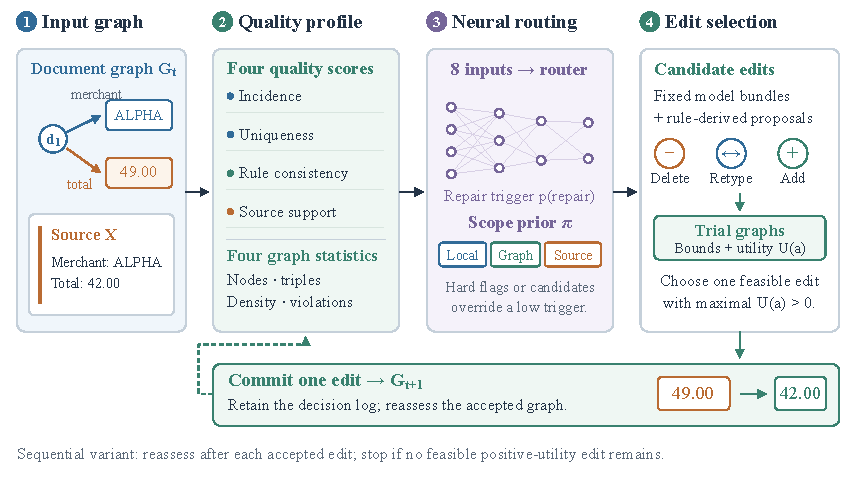
\includegraphics[width=0.98\textwidth]{figure/method/image1.pdf}
    \caption{用于编辑选择的尺度感知路由。评估概况和图统计量输入路由器，得到修复分数和三个编辑范围的权重。选择器在图副本上尝试模型与规则编辑，执行最佳允许正分编辑，再次检查。}
    \label{fig:framework_overview}
\end{figure}

\subsubsection{评估概况与共享输入}
\label{sec:impl:profile_revision}

选择器的评估概况使用四个分数，分别衡量节点连接、三元组唯一性、规则一致和来源支持：
\begin{equation}
\label{eq:quality_state}
\begin{split}
\mathbf{s}={}&(Q_{\mathrm{inc}},Q_{\mathrm{uniq}},Q_{\mathrm{rule}},Q_{\mathrm{src}}),\\
Q_i={}&100(1-r_i),\quad Q=\tfrac14\sum_i Q_i.
\end{split}
\end{equation}
每个 $r_i$ 是对应检查的错误率。对于非空图，各错误率为
\begin{equation}
\label{eq:profile_rates}
r_{\mathrm{inc}}=\frac{I}{n},\quad
r_{\mathrm{uniq}}=\frac{m-c}{m},\quad
r_{\mathrm{rule}}=\frac{B}{m},\quad
r_{\mathrm{src}}=\frac{V}{m}.
\end{equation}
$I$ 为无连接节点数，$c$ 为三元组相似组数。$B$ 为被图规则标记的不同三元组数。$V$ 为去掉空白后仍未在文本中出现的值的数量。这里，$n$、$m$ 分别为节点数和三元组数。这些分数为比较试改图提供统一尺度。空图的节点连接分为零，其余三项为 100。非空图没有源文本时，来源分为 50。

三元组相似度使用主体、关系和值的字符对计数。三部分余弦相似度的权重为 0.4、0.2、0.4。相似度达到 0.92 的三元组对组成相似组，用于唯一性评分。层级检查使用管理、监督和成员关系的方向，跳过含义不明确的关系。实体检查作用于标记为实体引用的端点，其他字段值按文本处理。

评估概况也报告来源字段缺失。来源字段检查读取文档、行或句子开头的允许标签之后的值。当原文给出一个字段而图中缺少它时，增加一个候选。重复标签给出冲突值时，跳过该字段。这些报告进入违规计数和候选列表。

路由器接收四项分数和四个图统计量：
\begin{equation}
\label{eq:routing_inputs}
\mathbf{g}=(n,m,\rho,n_{\mathrm{viol}}),\qquad
\rho=\frac{|E_{\mathrm{pair}}|}{n(n-1)}\quad(n>1).
\end{equation}
这里，$n$、$m$ 分别为节点数和三元组数。$E_{\mathrm{pair}}$ 包含不同的有向节点对，不含自连接。$n\leq1$ 时密度为零。$n_{\mathrm{viol}}$ 是报告的违规数。主报告 $D$ 列出字段错误，$\mathbf{s}$ 为选择器的图打分。两者都是评估概况，分别用于各自的修复路径。

\subsubsection{路由器与训练信号}

路由器将这八个输入转成修复分数和范围权重：
\begin{equation}
\label{eq:decision_net}
(p_{\mathrm{repair}},\boldsymbol{\pi})=
f_\phi(\operatorname{scale}([\mathbf{s};\mathbf{g}])).
\end{equation}
$\operatorname{scale}$ 使用训练集均值和标准差。$\boldsymbol{\pi}$ 有三个非负权重，合计为一，分别对应实体、图和上下文编辑。网络层大小为 $8\!\rightarrow\!32\!\rightarrow\!16$，具有一个修复输出和三个范围输出，共 884 个参数。两个隐藏层均使用 ReLU。sigmoid 给出修复分数，softmax 给出范围权重。训练和使用时共用特征代码。特征版本不匹配时，路由器改用等权重。

训练标签来自已知注入缺陷。损坏图的修复标签 $y_j$ 为一，其干净配对图的标签为零。范围标签 $c_j$ 取图中最常见的缺陷范围。干净图只训练修复输出。损失为
\begin{equation}
\label{eq:decision_loss}
\begin{split}
\mathcal L(\phi)={}&\frac1N\sum_j\operatorname{BCE}(p_j,y_j)\\
&+\frac{\sum_j b_j(-\log\pi_{j,c_j})}{\sum_j b_j+\epsilon}.
\end{split}
\end{equation}
有范围标签时，$b_j$ 为一；$\epsilon$ 避免除零。第一项训练修复分数，第二项用损坏图训练范围权重。同一文档组只属于训练、验证或测试中的一个划分。选择器根据任务输入和源文本计算特征。

\subsubsection{候选编辑与成本}
\label{sec:method:modalities}

规则和模型建议提供候选编辑。选择器可以删除三元组、改变关系或添加三元组。改变关系在代码中称为 retype。相关编辑可以组成一个包。在保存建议测试中，清理后输入与模型输出之间的差异按关系分组。每组是一个置信度为 0.7 的编辑包。

编辑成本鼓励小幅修改：
\begin{equation}
\label{eq:cost_hierarchy}
c(a)=\begin{cases}
0.30 & \text{删除},\\
0.16 & \text{改关系},\\
0.06 & \text{添加}.
\end{cases}
\end{equation}
编辑包的成本是其中各项编辑成本之和。这些固定成本与质量增益、范围权重一起进入试改分数。学习先验测试将路由器与始终开启的等权先验比较。

\subsection{试改检查与修复循环}
\label{sec:method:algorithm}

执行编辑前，先在图副本上试做每个候选。令 $G_a$ 为试改图，$h$ 为硬规则错误数，$\sigma(a)$ 为编辑范围，$z(a)$ 为候选置信度。默认分数为
\begin{equation}
\label{eq:action_utility}
\begin{split}
U(a)={}&\frac{Q(G_a)-Q(G)}{100}
+0.20\frac{\max(0,h(G)-h(G_a))}{\max(1,h(G))}\\
&-0.35c(a)+0.05\log\!\left(\max(\pi_{\sigma(a)},0.05)+10^{-6}\right)
+0.02z(a).
\end{split}
\end{equation}
各项分别衡量质量增益、规则错误减少、编辑成本、范围权重和候选置信度。试改重新计算完整图的评估概况，并检查分数边界、密度，以及编辑是否会把图删空。

四项分数的下界依次为 55、55、60、45。已经满足的下界必须继续满足。低于下界的分数必须保持或提高。在这些条件下，每项检查分数最多下降两分。试改后密度最多为 0.75，非空图必须保持非空。这些要求确定允许的试改集合 $\mathcal A_t^{\mathrm{ok}}$。选择步骤为
\begin{equation}
\label{eq:constrained_opt}
a_t^*=\arg\max_{a\in\mathcal A_t^{\mathrm{ok}}}U(a),\qquad U(a_t^*)>0.
\end{equation}
式~\ref{eq:constrained_opt}~在当前试改编辑中作出选择。边界决定哪些编辑允许执行，分数为允许编辑排序。没有允许编辑获得正分时，图保持原样。

\begin{figure}[t]
    \centering
    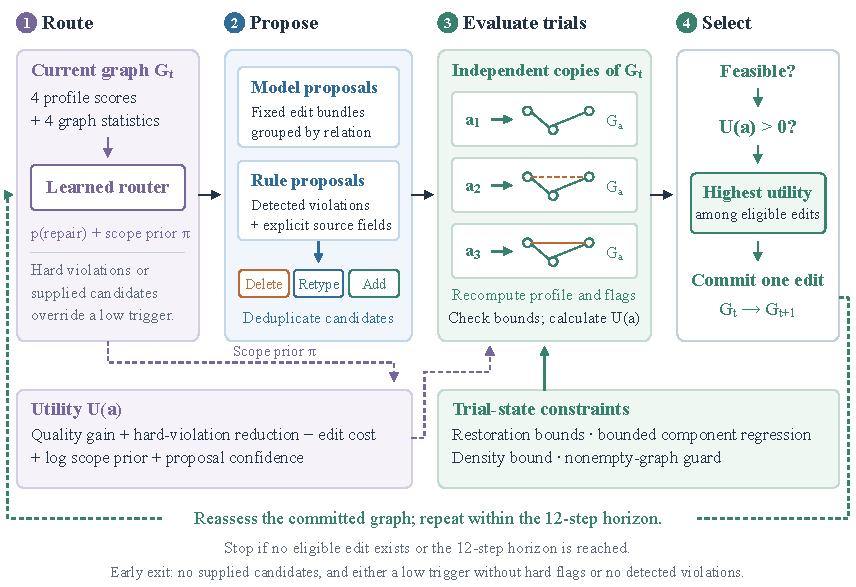
\includegraphics[width=0.98\textwidth]{figure/method/image3.pdf}
    \caption{一轮试改检查。路由器为编辑范围赋权，选择器在图副本上为每项模型或规则编辑打分、检查边界，并执行最佳允许正分编辑。随后重新构建评估概况。保存建议测试最多允许十二轮。}
    \label{fig:optimization_flow}
\end{figure}

算法~\ref{alg:enhancement}~连接评估、路由和执行。即使修复分数较低，只要存在已提供的候选或硬规则错误，也会开始试改检查。当没有有用的允许编辑、不再需要试改，或达到步数上限时，循环结束。日志保存试改图、分数、决策和停止原因。

\begin{algorithm}[t]
\caption{带试改检查的尺度感知编辑选择}
\label{alg:enhancement}
\begin{algorithmic}[1]
\Require 输入图 $G$、原文 $X$、已提供候选 $A_0$、任务输入、步数上限 $T$
\Ensure 修复图 $\widehat G$ 和决策日志 $J$
\State $\widehat G\gets G$; $J\gets\emptyset$; $E\gets\emptyset$
\State 将缺失来源字段的候选加入 $A_0$
\For{$t=1$ 到 $T$}
    \State 为 $\widehat G$ 计算评估概况和 $(p_{\mathrm{repair}},\boldsymbol\pi)$
    \If{$A_0=\emptyset$、$h(\widehat G)=0$ 且 $p_{\mathrm{repair}}<\tau_{\mathrm{repair}}$}
        \State \textbf{退出循环}
    \EndIf
    \If{没有报告的违规且 $A_0=\emptyset$}
        \State \textbf{退出循环}
    \EndIf
    \State $A\gets\textsc{Unique}(A_0\cup\textsc{RuleEdits}(\widehat G))$
    \State 跳过已在 $E$ 中的图与候选组合
    \State 对其余每个 $a\in A$ 在副本上试改，并将组合记入 $E$
    \State 为每次试改检查图边界并计算 $U(a)$
    \State 将试改分数和决策加入 $J$
    \If{没有允许候选满足 $U(a)>0$}
        \State \textbf{退出循环}
    \EndIf
    \State 对 $\widehat G$ 执行 $U(a)$ 最高的允许编辑
\EndFor
\State \Return $\widehat G,J$
\end{algorithmic}
\end{algorithm}

保存建议测试使用 $T=12$ 和 $\tau_{\mathrm{repair}}=0.05$。第二种评分从默认分数中减去 $0.05\log(1/3+10^{-6})$。这样，等权重的先验项为零。对于固定路由器，它保留编辑排序，但改变正分接受门槛。两种评分均在保存建议测试前固定。该选择器的来源匹配去掉两个字符串中的空白。档案也保留使用其他空白规则的早期日志。算法~\ref{alg:abstract}~和选择器分别测试。

对于 $m$ 条三元组，两两检查的成本为 $O(m^2)$。$T$ 轮、每轮最多 $K$ 次试改的成本为 $O(TKm^2)$，另加文本检查成本。主过滤器只扫描候选列表一次。


% Experiments
\section{实验评价}
\label{sec:eval}
\label{sec:experiments}

我们在注入缺陷、模型构建图、收据文本和合同字段上测试修复。共享提示用于测试上下文，过滤前后的评分用于测试门控，人工评审检查参考差异和实际编辑。本文提出三个问题：\textbf{RQ1}：修复何时能改善图？\textbf{RQ2}：上下文、过滤和编辑选择各改变了什么？\textbf{RQ3}：已有图何时比重新抽取更有用？表~\ref{tab:research_answers}~汇总结果。

\subsection{测试设置}
\label{sec:eval:setup}

\paragraph{来源记录与注入缺陷。}
来源数据包含陕西省人民政府的 4,728 条政务记录、国家金融监督管理总局的 1,000 条金融记录，以及生态环境部的 500 条环境记录。我们从每个来源最多抽取 500 篇文档，为每篇构建字段图。

源文本以“字段名：值”列出非空字段，用中文句号连接。每个值最多 320 个字符，服务标签最多 100 个字符。相同的清理后取值构成参考三元组。我们用随机种子 42，按 70/15/15 将文档划分为训练、验证和测试集。在加入缺陷前按来源编号划分，同一原始文档及其修改副本属于同一组。

每张测试图恰好加入两个缺陷。六种缺陷为三元组缺失、三元组重复、非法关系、反向边、无来源支持的值和层级冲突。保存的数据列出每条干净和修改后的三元组。测试集有 225 篇文档，每个来源 75 篇，共 450 个缺陷（表~\ref{tab:repair_benchmark}）。

\begin{table}[t]
\centering
\caption{注入缺陷测试数据。最后三列为文档数。}
\label{tab:repair_benchmark}
\small
\begin{tabular}{l r r r r r}
\toprule
领域 & 文档数 & 缺陷数 & 训练 & 验证 & 测试 \\
\midrule
政务 & 499 & 998 & 349 & 75 & 75 \\
金融 & 500 & 1,000 & 350 & 75 & 75 \\
环境 & 500 & 1,000 & 350 & 75 & 75 \\
\midrule
总计 & 1,499 & 2,998 & 1,049 & 225 & 225 \\
\bottomrule
\end{tabular}
\end{table}

\paragraph{模型构建的图。}
Claude Haiku 为相同的 225 篇测试文档分别构建新图。输入为源文本、文档编号和允许关系。评分器将结构化字段作为参考值。十个响应的 JSON 无效，按空图计分，解析成功率为 95.56\%。共有 77 张图与参考不同，包含 302 项三元组差异。两名评审检查其中固定抽样的 200 项差异，第三名评审解决分歧（第~\ref{sec:eval:human}~节）。

\paragraph{修复方法。}
所有方法获得相同输入图、源文本、文档编号和允许关系。
\begin{itemize}
    \item \textbf{来源字段复制}：读取字段标签，直接从文本复制值。
    \item \textbf{不修复}：返回输入。
    \item \textbf{仅规则}：去重，将指向文档节点的边反向，删除非法头节点和关系。
    \item \textbf{SHACL 风格修复}：使用 SHACL 形状约束检查文档头节点和允许关系\citep{ref_shacl2017}。
    \item \textbf{直接调用模型}：调用一次模型，根据原文返回完整图。
    \item \textbf{ReAct 风格智能体}：一次调用查找错误，另一次调用执行修复\citep{ref_yao2023react}。
    \item \textbf{简单流程}：清理输入，调用一次模型，并对响应去重。
    \item \textbf{诊断＋门控}：在提示中增加错误报告，按文档编号、关系、来源匹配、重复数量和每字段值数量过滤输出。
\end{itemize}

除另行指定模型外，模型方法均在同一端点使用 \texttt{claude-haiku-4-5-20251001}\citep{ref_anthropic_claude45}，温度为零。所有分数均包含失败调用。注入缺陷测试中，直接调用模型 和 简单流程 各有一个无效 JSON 响应，诊断＋门控 和 ReAct 均为零。

\paragraph{评分与统计检验。}
当输出恢复各条干净三元组的数量，并去掉其修改形式时，该缺陷视为修复。我们还衡量正确事实保留、过度修复、三元组 F1、整图精确匹配、调用次数和请求时间。整图精确匹配同时检查三元组与重复数量。

令 $G_0$ 为模型构建的输入图，$G_1$ 为修复图，$G^*$ 为参考图。令 $d$ 统计多余和缺失的三元组，包括重复副本。参考差异减少率为
\[
    1-\frac{d(G_1,G^*)}{d(G_0,G^*)},
\]
该指标在 77 个与参考不同的输入上取平均。负值表示输出差异变多。事实保留和过度修复也按参考三元组计算。人工分数衡量评审是否发现错误、是否接受编辑。

置信区间（CI）使用 10,000 次配对 bootstrap 抽样。匹配测试每次抽取完整文档，使同一文档的两个注入缺陷保持在一起。配对符号随机化检验使用 10,000 次抽样和种子 42。较早的缺陷与整图匹配比较使用精确 McNemar 检验。模型输出差异数还使用单侧配对 Wilcoxon 检验。

首次匹配上下文测试使用未校正的 $p$ 值。后续组件、收据上下文和保存响应测试按各表所列分组进行 Holm 校正。每个 95\% 置信区间对应一个比较，Holm 校正作用于同一检验组的 $p$ 值。

\subsection{注入缺陷修复}
\label{sec:eval:overall}

诊断＋门控 修复 98.00\% 的缺陷，保留 99.32\% 的干净事实，F1 达 99.17\%（表~\ref{tab:repair_main}）。简单流程 使用相同的一次调用上限，修复率为 95.11\%，F1 为 96.34\%。诊断＋门控 修复了 简单流程 漏掉的 15 个缺陷；简单流程 修复了 诊断＋门控 漏掉的两个缺陷（McNemar $p=0.00235$）。配对修复率增益为 2.89 个百分点（95\% 置信区间：1.11--4.89；$p=0.0067$），F1 增益为 2.84 个百分点（95\% 置信区间：1.65--4.25）。直接调用模型 的修复率为 92.44\%。来源字段复制 直接读取记录中的字段名和值，不调用模型，修复率和整图匹配均为 100\%。

\begin{table*}[t]
\centering
\caption{225 篇测试文档、450 个注入缺陷上的修复结果。过度修复、调用数和请求时间越低越好。}
\label{tab:repair_main}
\small
\resizebox{\textwidth}{!}{%
\begin{tabular}{l c c c c c c c}
\toprule
方法 & 缺陷修复 & 事实保留 & 过度修复 & 三元组 F1 & 整图匹配 & 调用／篇 & 耗时／篇 \\
\midrule
来源字段复制 & \textbf{1.0000} & \textbf{1.0000} & \textbf{0.0000} & \textbf{1.0000} & \textbf{1.0000} & 0.00 & $<0.001$ s \\
不修复 & 0.0000 & \textbf{1.0000} & \textbf{0.0000} & 0.7615 & 0.0000 & 0.00 & $<0.001$ s \\
仅规则 & 0.3200 & \textbf{1.0000} & \textbf{0.0000} & 0.8472 & 0.0622 & 0.00 & $<0.001$ s \\
SHACL 风格修复 & 0.0000 & \textbf{1.0000} & \textbf{0.0000} & 0.7998 & 0.0000 & 0.00 & $<0.001$ s \\
直接调用模型 & 0.9244 & 0.9687 & 0.0758 & 0.9520 & 0.8267 & 1.00 & 7.25 s \\
ReAct 风格智能体 & 0.8911 & 0.9324 & 0.1667 & 0.9213 & 0.5956 & 2.00 & 20.50 s \\
简单流程 & 0.9511 & 0.9723 & 0.0705 & 0.9634 & 0.8400 & 1.00 & 9.27 s \\
诊断＋门控 & 0.9800 & 0.9932 & 0.0167 & 0.9917 & 0.9333 & 1.00 & 11.44 s \\
\bottomrule
\end{tabular}%
}
\end{table*}

诊断＋门控 修复了 直接调用模型 漏掉的 28 个缺陷；直接调用模型 修复了 诊断＋门控 漏掉的三个缺陷（$p=4.65\times10^{-6}$）。与 ReAct 比较时，两项计数分别为 42 和二（$p=1.13\times10^{-10}$）。这些检验比较完整修复方法，第~\ref{sec:eval:mechanisms}~节再测试其中步骤。

\begin{figure*}[t]
\centering
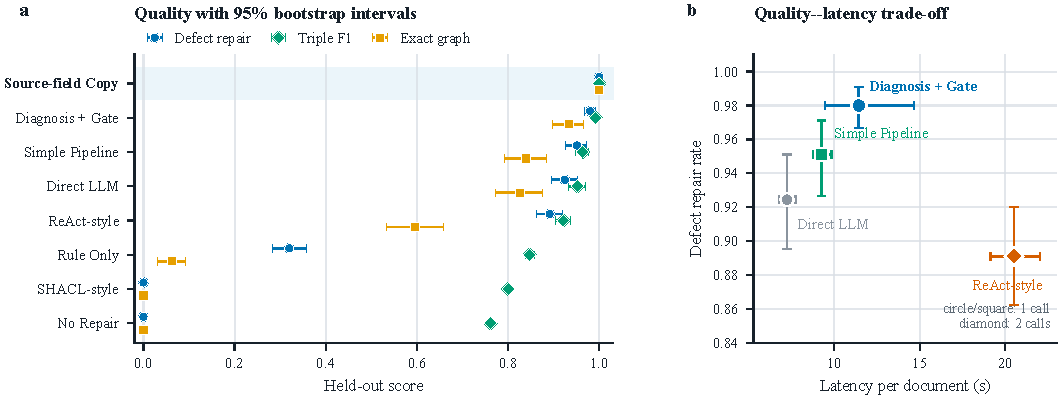
\includegraphics[width=0.98\textwidth]{figure/experiments/repair_benchmark_results.pdf}
\caption{注入缺陷修复。\textbf{a}：修复率、三元组 F1 和整图匹配，带基于文档抽样的 95\% 置信区间。\textbf{b}：一次或两次调用方法的分数与请求时间。}
\label{fig:repair_benchmark_results}
\end{figure*}

\subsection{模型构建图的修复}
\label{sec:eval:natural}

输入图的 F1 为 87.99\%，整图匹配为 65.78\%（表~\ref{tab:natural_errors}）。诊断＋门控 将 F1 提高到 92.48\%，参考差异减少 27.75\%，并保留全部原本匹配参考的输入三元组。简单流程 在 77 个有差异输入上的平均差异减少率为 $-59.15\%$，增加的差异多于去掉的差异。

诊断＋门控 的 F1 比 简单流程 高 4.40 个百分点（95\% 置信区间：3.07--5.77），平均每篇少 1.03 项差异（95\% 置信区间：0.77--1.32；Wilcoxon $p=3.18\times10^{-12}$）。三个图在 诊断＋门控 下完全匹配参考，在 简单流程 下不匹配；反向情况为零（$p=0.25$）。来源字段复制 匹配全部参考。

\begin{table*}[t]
\centering
\caption{模型构建图的修复。差异减少率使用 77 个与参考不同的输入，其余分数使用全部 225 篇文档。}
\label{tab:natural_errors}
\small
\resizebox{\textwidth}{!}{%
\begin{tabular}{l c c c c c c c}
\toprule
方法 & 解析率 & 非精确输入 & 差异减少率 & 事实保留 & 过度修复 & 三元组 F1 & 整图匹配 \\
\midrule
来源字段复制 & 1.0000 & 77 & 1.0000 & 1.0000 & 0.0000 & 1.0000 & 1.0000 \\
抽取图，不修复 & 0.9556 & 77 & 0.0000 & 1.0000 & 0.0000 & 0.8799 & 0.6578 \\
简单流程 & 1.0000 & 77 & $-0.5915$ & 0.9971 & 0.2389 & 0.8807 & 0.6711 \\
诊断＋门控 & 0.9956 & 77 & 0.2775 & 1.0000 & 0.0292 & 0.9248 & 0.6844 \\
\bottomrule
\end{tabular}%
}
\end{table*}

\paragraph{有效与无效 JSON 输入。}
215 个有效 JSON 输入的 F1 为 92.09\%。诊断＋门控 达到 93.53\%，简单流程 为 88.85\%。67 个有效但有参考差异的输入中，诊断＋门控 使差异减少 24.00\%，F1 从 74.61\% 提高到 79.22\%。148 个原本精确匹配的图全部保持精确匹配。十个无效输入修复后的 F1 为 69.91\%，没有一个整图精确匹配。

\begin{figure}[t]
\centering
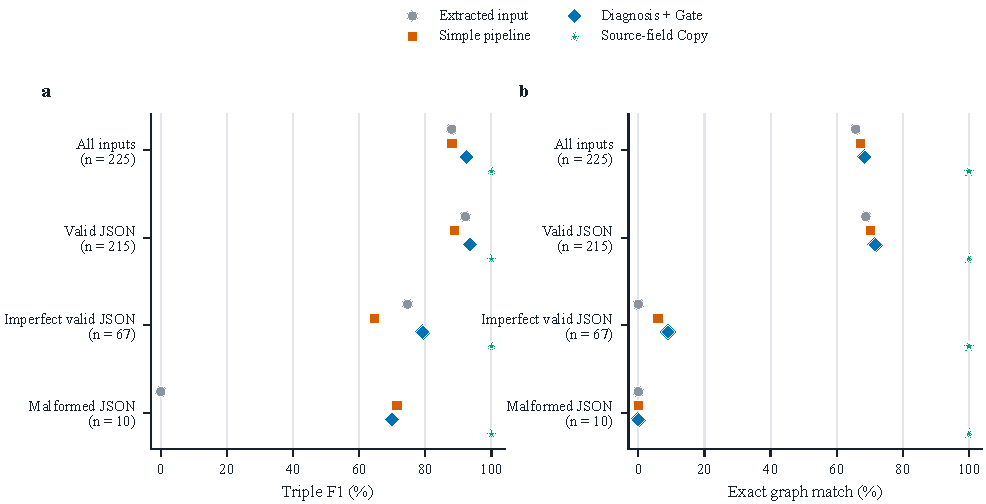
\includegraphics[width=0.98\textwidth]{figure/experiments/natural_stratified.pdf}
\caption{按输入类型划分的修复分数。有效 JSON 组展示可解析图的修复，无效 JSON 组展示空输入的恢复。}
\label{fig:natural_stratified}
\end{figure}

\subsection{提示、过滤与编辑选择器测试}
\label{sec:eval:router}
\label{sec:eval:mechanisms}

我们依次测试提示文本、过滤和编辑选择。在保存的 Claude 响应上，过滤将 F1 从 98.95\% 提高到 99.17\%，过度修复降低 0.60 个百分点。修复率保持 98.00\%，整图匹配保持 93.33\%。过滤器去掉八条三元组，均未通过来源检查且与参考不同。附录~\ref{sec:eval:ablation}~给出完整方法表。

% Begin merged sections/audit_primary.tex
% Generated by exps/paper1_mechanism_audit/write_paper_tables.py
\begin{table*}[t]
\centering
\caption{Gemma 提示测试，每组输入 60 篇文档。每个原始／过滤对照使用同一响应。}
\label{tab:matched_mechanisms}
\small
\resizebox{\textwidth}{!}{%
\begin{tabular}{llrrrr}
\toprule
上下文 & 输出 & 受控修复 & 受控 F1 & 模型构建 F1 & 模型构建整图匹配 \\
\midrule
基础提示 & 未过滤 & 0.9750 & 0.9951 & 0.9185 & 0.6667 \\
基础提示 & 门控 & 0.9750 & 0.9962 & 0.9252 & 0.6667 \\
诊断提示 & 未过滤 & 0.9250 & 0.9850 & 0.9079 & 0.6667 \\
诊断提示 & 门控 & 0.9250 & 0.9861 & 0.9147 & 0.6667 \\
SHACL 上下文 & 未过滤 & 0.9500 & 0.9912 & 0.9322 & 0.7000 \\
SHACL 上下文 & 门控 & 0.9500 & 0.9912 & 0.9364 & 0.7000 \\
\bottomrule
\end{tabular}%
}
\end{table*}
% End merged sections/audit_primary.tex


Gemma 测试使用 60 篇文档，每个来源 20 篇，分别测试注入缺陷输入和模型构建输入。三个提示共享指令、清理步骤、温度和输出上限。每个响应在同一门控过滤前后计分。表~\ref{tab:matched_mechanisms}~给出六种设置，表~\ref{tab:matched_cost}~给出输入 token 数和请求时间。第~\ref{sec:impl:shacl}~节给出 SHACL 提示。

经过过滤，基础提示在注入缺陷输入上达到 99.62\% F1 和 97.50\% 修复率。错误报告提示为 98.61\% F1 和 92.50\% 修复率。配对 F1 变化为 $-1.01$ 个百分点（95\% 置信区间：$[-1.67,-0.38]$；$p=0.0082$）。模型构建输入上，基础提示 + 门控 的 F1 为 92.52\%，诊断＋门控 为 91.47\%，SHACL 上下文＋门控 为 93.64\%。诊断 与 SHACL 的 F1 差为 $-2.16$ 个百分点（95\% 置信区间：$[-5.26,0.02]$；$p=0.105$）。

在使用错误报告提示的模型构建输入上，过滤将 F1 从 90.79\% 提高到 91.47\%，增益为 0.69 个百分点（95\% 置信区间：0.20--1.29；$p=0.0335$），整图匹配保持相同。360 个响应共拒绝 27 条三元组，均与参考不同。

\begin{figure}[t]
\centering
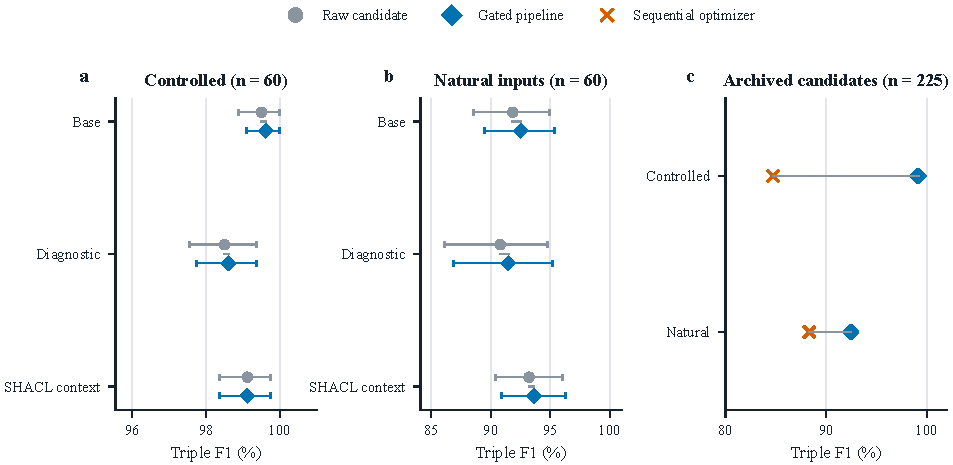
\includegraphics[width=0.98\textwidth]{figure/experiments/matched_mechanisms.pdf}
\caption{提示、过滤和选择器测试。a--b 使用 60 篇文档的 Gemma 输出；每个原始／过滤对照使用同一响应，误差线表示 95\% 文档 bootstrap 置信区间。c 使用 225 篇文档保存的 Claude 建议。}
\label{fig:matched_mechanisms}
\end{figure}

% Begin merged sections/factorial_controls.tex
\paragraph{联合测试清理、错误报告与过滤。}
\label{sec:eval:factorial}

我们分别开启或关闭输入清理（$P$）与错误报告（$D$）。四种提示设置使用 60 个注入缺陷输入和 60 个模型构建输入，得到 480 个 Gemma 响应。每个响应分别在启用和关闭门控（$G$）时计分。每项主效应都对另外两个开关取平均。

\begin{table}[t]

\centering

\caption{平均 F1 变化，单位为百分点。每组输入有 60 篇配对文档，各效应对另外两个开关取平均。区间为 95\% 文档 bootstrap 置信区间。$p_H$ 对六项主效应检验进行 Holm 校正。}
\label{tab:recovery_factorial}

\small

\begin{tabular}{llrrr}

\toprule

输入 & 组件 & 变化 & 95\% 区间 & $p_H$ \\

\midrule

受控输入 & 预处理 & -0.028 & [-0.797, 0.778] & 1.000 \\

受控输入 & 诊断 & -0.651 & [-1.348, -0.056] & 0.164 \\

受控输入 & 门控 & +0.164 & [0.054, 0.301] & 0.156 \\

模型构建输入 & 预处理 & +0.697 & [0.000, 1.905] & 1.000 \\

模型构建输入 & 诊断 & -0.535 & [-2.376, 0.842] & 1.000 \\

模型构建输入 & 门控 & +0.707 & [0.225, 1.316] & 0.086 \\

\bottomrule

\end{tabular}

\end{table}

六项 Holm 校正后的 $p$ 值均大于 0.05（表~\ref{tab:recovery_factorial}）。错误报告在两组输入中都降低平均 F1。门控在注入缺陷输入上提高 0.164 个百分点，在模型构建输入上提高 0.707 个百分点。所有输入组共拒绝 47 条三元组，其中 17 条文档编号错误，30 条未通过来源匹配，均与参考不同。公开分数还列出开关联合效应和每项检查去掉的候选。


\paragraph{各项过滤检查。}
我们将 540 个已保存响应经过八种过滤设置，得到 4,320 个输出。完整过滤器拒绝 28 条三元组，其中 11 条文档编号错误，17 条来源匹配失败，均与参考不同。其他检查在该样本中未额外去掉候选。21 项检查比较的校正后 $p$ 值均大于 0.05。附录~\ref{sec:eval:individual_ablation}~给出结果表。

\paragraph{编辑选择。}
在保存的 Claude 建议上，默认选择器无论使用学习权重还是等权重，在注入缺陷输入上都接受零项编辑。修复率保持 32.00\%，F1 保持 84.72\%，与清理后输入相同。v2 运行中，模型构建输入的等权重 F1 为 88.33\%，学习权重为 87.99\%，学习触发器也为 87.99\%。去掉编辑成本将注入缺陷 F1 提高到 89.30\%，该设置的模型构建 F1 为 88.13\%。日志显示，一些评估分数较高的图仍缺少字段。某些有用的添加得到不大于零的分数，因而被拒绝。附录~\ref{sec:eval:individual_ablation}~给出全部 13 种设置、两种先验评分形式和 11,700 个结果。附录~\ref{app:historical_diagnostics}~还给出早期选择器结果和调用策略测试。

\subsection{两个模型的测试}
\label{sec:eval:crossmodel}

我们在 60 个注入缺陷输入上比较 直接调用模型、简单流程 和 诊断＋门控，每个来源 20 个。模型为 Claude Haiku 和 \texttt{google/gemma-4-26B-A4B-it}\citep{ref_gemma4}。每种方法跨模型使用相同输入、提示形式、温度和一次调用上限。诊断＋门控 在两个模型上的修复率均最高（表~\ref{tab:cross_model}）。它相对 简单流程 的 F1 优势在 Claude 上更大。Gemma 直接输出的 F1 高于 Claude。

\begin{table}[t]
\centering
\caption{两个模型在相同 60 个注入缺陷输入上的结果。}
\label{tab:cross_model}
\small
\begin{tabular}{l l c c c}
\toprule
模型 & 方法 & 修复率 & F1 & 精确匹配 \\
\midrule
Claude & 直接 & 0.958 & 0.970 & 0.867 \\
Claude & 简单流程 & 0.958 & 0.966 & 0.833 \\
Claude & \textbf{诊断＋门控} & \textbf{0.975} & \textbf{0.991} & \textbf{0.917} \\
\midrule
Gemma & 直接 & 0.958 & 0.988 & 0.883 \\
Gemma & 简单流程 & 0.967 & 0.984 & 0.867 \\
Gemma & \textbf{诊断＋门控} & \textbf{0.983} & \textbf{0.990} & \textbf{0.917} \\
\bottomrule
\end{tabular}
\end{table}

% Begin merged sections/receipt_followup.tex
\subsection{新收据上的来源行提示}
\label{sec:eval:receipt_followup}

首次 60 张收据测试中，基础提示和错误报告提示都保留全部输入图不变。过滤将 F1 从 79.44\% 降到 79.15\%。一个地址因空白与来源不同而被拒绝。49 项参考差异中，有 27 项涉及大小写、空白、标点或金额格式（附录~\ref{sec:eval:external_receipts}）。据此，我们加入字段含义、来源行提示和共享空白规则。

我们用 20 张新收据设置索引设计，然后固定设计，在另外 60 张收据上测试（第~\ref{sec:framework:field_evidence}~节）。首次 60 张、开发 20 张和新测试 60 张收据的编号不同，空白清理后的文本也不同。抽样种子为 20260923。所有预测保存后才下载测试标签。每种方法得到相同字段含义、带行号原文、输入图和指令。简单流程 直接使用这些输入；证据索引 增加字段行提示；SHACL 增加规则检查上下文。三种方法的过滤器使用相同空白规则。

开发集 F1 为：输入 80.00\%，简单流程 82.50\%，证据索引 85.00\%，SHACL 80.00\%。测试保留一个索引设计和全部三种方法。主要比较为 证据索引 减 简单流程 的文档平均 F1。代码和评分规则在测试前固定。

\begin{table*}[t]
\centering
\caption{60 张新收据的修复。各方法共享字段含义、来源行和空白检查。精确匹配使用有标签字段。}
\label{tab:receipt_followup}
\small
\begin{tabular}{lrrrr}
\toprule
方法 & 三元组 F1 & 整图匹配 & 规范化 F1 & 事实保留 \\
\midrule
抽取输入 & 0.7833 & 0.3500 & 0.7958 & 1.0000 \\
简单流程, 未过滤 & 0.7875 & 0.2833 & 0.8083 & 0.9250 \\
简单流程, 过滤后 & 0.7875 & 0.2833 & 0.8083 & 0.9250 \\
证据索引, 未过滤 & 0.8333 & 0.4000 & 0.8625 & 0.9306 \\
证据索引, 过滤后 & 0.8351 & 0.4000 & 0.8643 & 0.9306 \\
SHACL 上下文，未过滤 & 0.7833 & 0.2833 & 0.8042 & 0.9347 \\
SHACL 上下文，过滤后 & 0.7833 & 0.2833 & 0.8042 & 0.9347 \\
\bottomrule
\end{tabular}
\end{table*}

新测试集的输入 F1 为 78.33\%。过滤后 简单流程、证据索引、SHACL 分别为 78.75\%、83.51\%、78.33\%。简单流程 比输入高 $0.42$ 个百分点（95\% 置信区间：$[-4.17,5.00]$）。证据索引 比 简单流程 高 $4.76$ 个百分点（95\% 置信区间：$[2.50,7.26]$；配对随机化 $p=0.0004$）。三种方法的整图匹配分别为 28.33\%、40.00\%、28.33\%。

输入有 52 个字段与参考不同。简单流程 恢复其中 16 个，并丢失 15 个原本精确匹配的字段。证据索引 恢复 26 个、丢失 14 个；SHACL 恢复 13 个、丢失 13 个。索引修正了 11 项标点差异和 6 项文本边界差异。它丢失的 14 个精确匹配中，有 10 个数值金额相同，只改变显示格式。

金额检查去掉总额字段中的货币前缀和千位分隔符。正确金额数为：输入 58/60，简单流程 59/60，证据索引 59/60，SHACL 58/60。清理大小写和空白后，证据索引 的 F1 为 86.43\%，简单流程 为 80.83\%。索引同时提高精确和清理后文本分数。

过滤器拒绝 1 个候选。它与参考不同，并将地址片段拼成原文中没有的文本。被拒绝的参考匹配候选数为 0。过滤使索引 F1 提高 0.18 个百分点，另外两种方法的 F1 保持不变。

简单流程、证据索引、SHACL 分别修改 31、39、28 个输入图。平均修复请求时间为 7.91、7.88、8.11 秒，平均输入长度为 1784、2153、3404 个 token。240 次请求产生 60 个抽取输出和 180 个修复输出。请求时间包含间隔等待和重试。每个原始与过滤后评分对只使用一个响应。

\begin{figure}[t]
\centering
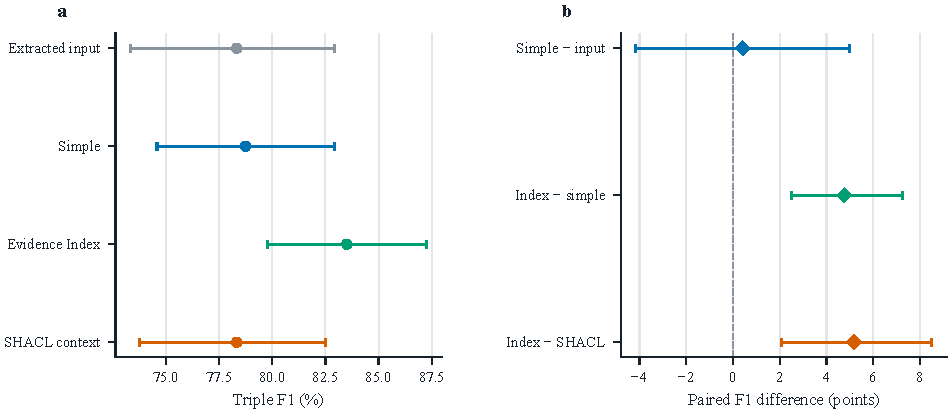
\includegraphics[width=0.98\textwidth]{figure/experiments/receipt_followup.pdf}
\caption{新收据测试。左：平均 F1 及 95\% 文档 bootstrap 置信区间。右：配对 F1 变化。所有方法共享字段含义和来源行。}
\label{fig:receipt_followup}
\end{figure}
% End merged sections/receipt_followup.tex

% Begin merged sections/receipt_context_controls.tex
\subsection{来源行提示对照}
\label{sec:eval:recovery_ablation}

我们在相同 60 张新测试收据上比较六种提示设置。测试使用与组件测试同批的 360 个新 Gemma 响应，全部解析成功。各设置都保留完整原文，并共享模型、输出上限和过滤器。随机索引的字符长度与完整索引大致相同。

\begin{table}[t]

\centering

\caption{60 张收据上的来源行测试。各行使用相同模型、原文、输出上限和过滤器。随机提示与索引的字符长度大致相同。}
\label{tab:recovery_index}

\small

\begin{tabular}{lrr}

\toprule

上下文 & 精确 F1 & 规范化 F1 \\

\midrule

简单流程 & 0.7917 & 0.8125 \\

完整索引 & 0.8351 & 0.8643 \\

仅锚点 & 0.8351 & 0.8643 \\

随机索引 & 0.8167 & 0.8458 \\

简单流程，无字段定义 & 0.8083 & 0.8292 \\

完整索引，无字段定义 & 0.7470 & 0.7762 \\

\bottomrule

\end{tabular}

\end{table}

完整索引的 F1 比 简单流程 高 4.35 个百分点（95\% 置信区间：1.25 至 7.86）。五项预设比较的 Holm 校正值为 $p_H=0.065$。完整索引与仅锚点行的平均 F1 相同。完整索引与随机索引相差 1.85 个百分点（置信区间：$[-0.65,4.52]$；$p_H=0.696$）。去掉字段含义使完整索引 F1 下降 8.81 个百分点（置信区间：$[4.23,13.39]$；$p_H=0.006$）。本批次 简单流程 去掉字段含义后得分更高。这些结果说明字段含义有助于索引提示选择取值。

\begin{figure}[t]

\centering

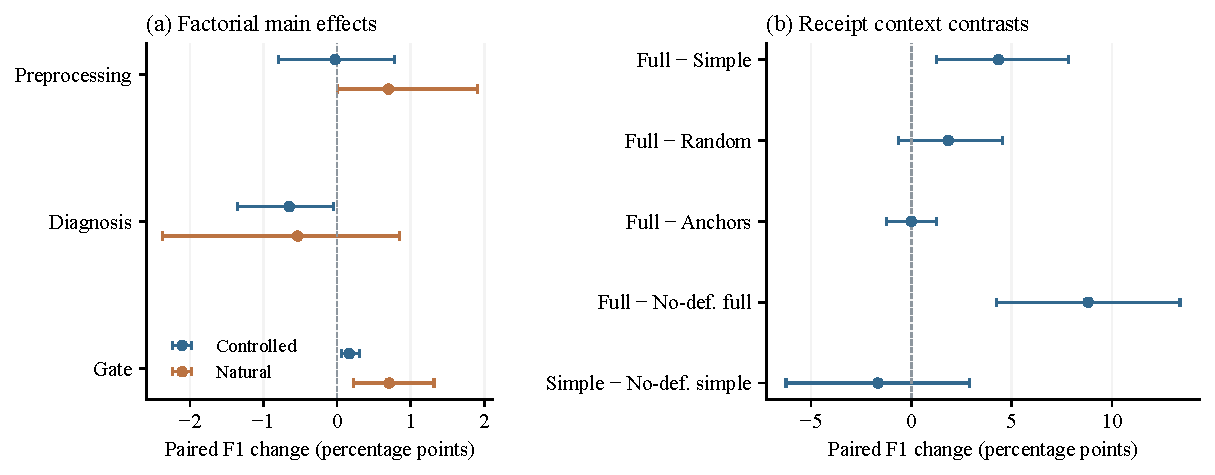
\includegraphics[width=0.98\textwidth]{figure/experiments/recovery_ablation.pdf}

\caption{组件与来源行测试。点表示平均配对 F1 变化，误差线为各项变化的 95\% 置信区间。组件测试与收据测试分别进行 Holm 校正。}
\label{fig:recovery_ablation}

\end{figure}
% End merged sections/receipt_context_controls.tex

% Begin merged sections/reextraction_recovery.tex
\subsection{修复与重新抽取}
\label{sec:eval:reextraction}

我们复用 60 张新测试收据，比较有无索引下的修复与重新抽取，共四种设置。各设置共享来源行、字段含义、文档编号和输出上限；修复额外获得已有图。全部 240 个响应都将 JSON 放在 Markdown 代码围栏中，固定的严格解析器将其计为失败。

随后，我们去掉代码围栏，并为每个输出指定已知文档编号，对相同响应重新计分。这项补充分析得到索引修复 F1 为 83.93\%，索引重新抽取为 74.86\%，配对差为 9.07 个百分点（95\% 置信区间：5.22 至 13.10）。修复调用使用已有图，其构建成本另计。附录~\ref{app:reextraction_diagnostics}~给出严格评分、围栏清理评分、编号错误和来源行覆盖。合同测试在采集前固定围栏处理和编号分配。

% Begin merged sections/cuad_contracts.tex
\subsection{合同字段测试}
\label{sec:eval:cuad}

我们用 CUAD\citep{ref_cuad} 测试五个字段：文档名称、签约日期、生效日期、到期日期或初始期限，以及适用法律。选择空白清理后每字段最多一个不同参考值、原文不超过 40,000 字符的合同。保留完整原文，并检查标注值的位置。20 份官方训练合同构成开发集；全部 56 份满足规则的官方测试合同构成测试集。

比较初始抽取、简单流程 修复、索引修复和索引重新抽取。两种修复方法得到相同初始图，索引方法在完整原文之外增加字段行窗口。各设置共享 Gemma 模型、字段含义和 4,000 token 输出上限。采集前，程序已设置 JSON 围栏处理和文档编号分配。一轮开发之后，提示与选择规则保持固定。

\begin{table}[t]
\centering
\caption{56 份文档的合同结果。F1 检查空白清理后的精确文本。“丢失”统计被删除的正确输入事实。输入行给出初始图成本，修复行给出修复调用成本。}
\label{tab:cuad}
\small
\begin{tabular}{lrrrr}
\toprule
输出 & F1 (\%) & 丢失 & 新增不匹配 & 请求数 \\
\midrule
初始抽取 & 46.76 & 0 & 0 & 59 \\
简单流程修复 & 43.35 & 7 & 2 & 71 \\
索引修复 & 44.84 & 5 & 12 & 69 \\
索引重新抽取 & 44.12 & 8 & 32 & 71 \\
\bottomrule
\end{tabular}
\end{table}

索引修复 F1 为 44.84\%，输入为 46.76\%，下降 1.92 个百分点。它删除五条正确输入事实，并增加十二条与参考不同的事实。简单流程 修复也低于输入。

索引修复的 F1 比索引重新抽取高 0.72 个百分点（95\% 配对置信区间：[-4.80,6.48]；符号翻转检验 $p=0.810$）。测试共用 270 次请求得到 224 个输出，包括重试。失败输出计为空图。评分在空白清理后，将复制文本与 CUAD 标签比较。

\begin{figure}[t]
\centering
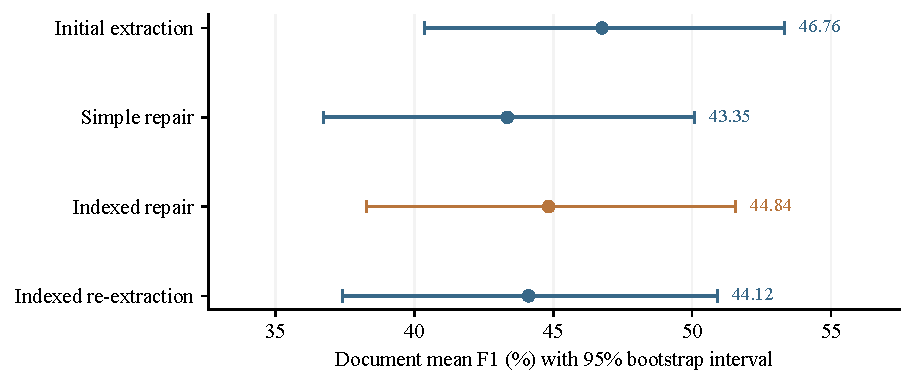
\includegraphics[width=0.88\textwidth]{figure/experiments/cuad_contracts.pdf}
\caption{合同分数。点表示文档平均 F1，误差线为各方法的 95\% 置信区间。正文给出修复与抽取的配对差值区间。}
\label{fig:cuad}
\end{figure}
% End merged sections/cuad_contracts.tex


\subsection{错误与编辑的人工评价}
\label{sec:eval:human}

任务 D 从模型构建输入的 302 项三元组差异中抽取 200 项参考差异。任务 E 从五种设置的 598 项编辑中抽取 200 项实际编辑。两者都用种子 42 随机抽样。每项是一项差异或编辑，同一文档可提供多项。评审看到原文、模式、输入图和指定操作。任务 E 还展示完整输出图。方法名称与参考质量提示隐藏。

两名具有计算机背景和中文阅读能力的评审先阅读规则和练习样例，再各自独立标注相同的 400 项。每项回答两个问题：输入在该位置是否有错（\texttt{is\_error}），以及添加或删除操作是否可接受（\texttt{repair\_acceptable}）。标签为 0、1 或 U，并说明理由。U 表示所示证据不足以作出判断。第三名评审检查原文和图，在两人的答案中选择，解决 154 项分歧。其余 246 项保留一致标签。一项编辑接受判断仍为 U。原始标签和一致性分数均保留。

\begin{table}[t]
\centering
\caption{人工评分。一致率和 $\kappa$ 使用两位评审原始的 0/1/U 答案。正例数使用最终标签，接受率使用答案为 0 或 1 的项目。}
\label{tab:human_review}
\small
\begin{tabular}{llrrrr}
\toprule
任务 & 判断 & 一致率 & $\kappa$ & 正例／确定项 & U \\
\midrule
D & 输入错误 & 80.0\% & 0.600 & 95/200 (47.5\%) & 0 \\
D & 建议编辑可接受 & 62.0\% & 0.334 & 86/200 (43.0\%) & 0 \\
E & 输入错误 & 86.0\% & 0.677 & 134/200 (67.0\%) & 0 \\
E & 实际编辑可接受 & 65.0\% & 0.128 & 134/199 (67.3\%) & 1 \\
\bottomrule
\end{tabular}
\end{table}

评审在 95/200 项参考差异中发现输入错误，接受 86/200 项建议编辑，以及 134/199 项实际编辑，另有一项不确定。一个缺失值本身可以是正确的，但添加后可能使仅允许一个值的字段出现两个值。输入错误与编辑接受问题分别覆盖这两个判断。任务 E 的原始编辑一致率为 65.0\%，$\kappa=0.128$。

\begin{table}[t]
\centering
\caption{按设置划分的实际编辑接受率。随机样本的各组大小不同，比例使用有明确判断的编辑。}
\label{tab:human_review_by_config}
\small
\begin{tabular}{lrrr}
\toprule
配置 & 抽样数 & 可接受 & U \\
\midrule
历史简单流程 & 105 & 63/104 (60.6\%) & 1 \\
历史诊断＋门控 & 41 & 25/41 (61.0\%) & 0 \\
Gemma 基础提示＋门控 & 16 & 13/16 (81.3\%) & 0 \\
Gemma 诊断＋门控 & 16 & 13/16 (81.3\%) & 0 \\
Gemma SHACL 上下文＋门控 & 22 & 20/22 (90.9\%) & 0 \\
\bottomrule
\end{tabular}
\end{table}

样本包含 105 项 历史简单流程 编辑、41 项 历史诊断＋门控 编辑、16 项 Gemma 基础提示＋门控 编辑、16 项 Gemma 诊断＋门控 编辑，以及 22 项 Gemma SHACL 上下文＋门控 编辑。表中按各组报告被接受编辑的比例。

\subsection{讨论}
\label{sec:eval:failure}

来源格式影响修复方法的选择。对于列出字段名和值的记录，解析器可以直接复制字段；收据则需要从全文中选择取值。新收据测试中，来源行提示提高 F1。后续索引测试展示字段含义的作用：去掉后，索引 F1 下降 8.81 个百分点。合同索引修复 F1 为 44.84\%，输入为 46.76\%。保留正确输入字段是清楚的改进目标。

实验还展示过滤器改变了什么。来源和文档编号检查去掉多余三元组。字段选择发生在模型生成和首值规则中。例如，来源可能同时包含小计和最终金额，修复方法必须为“total”选出正确的一个。因此，检查需要同时考虑关系含义和取值是否出现在原文中。

人工评审接受五种设置合并样本中 67.3\% 的编辑，并在 47.5\% 的参考差异样本中发现输入错误。历史诊断＋门控 样本中，接受的编辑为 25/41。结合原始标签和理由，这些分数帮助定位字段选择与单项编辑决策中的错误。

\subsection{代码与数据}

代码、提示、数据名单、模型输出和评分脚本位于 \url{https://github.com/turambar928/MCP_based_KG_construction}。每次运行保存模型设置、解析状态、请求和 token 用量，全部响应均保留。各实验 README 给出数据来源、样本、校验值和运行命令。

人工评价文件包含固定任务规则、评分器、汇总结果、原始一致性分数和样本名单。个人答案与理由不公开。收据评分使用 SROIE 的人工字段标签。

\begin{table}[t]
\centering
\caption{研究问题与测试结果。}
\label{tab:research_answers}
\small
\begin{tabularx}{\textwidth}{@{}p{0.10\textwidth}XX@{}}
\toprule
问题 & 比较 & 结果 \\
\midrule
RQ1 & 注入缺陷与模型构建图
& 诊断＋门控改善修复率和 F1。直接复制匹配全部中文记录参考。 \\
RQ2 & 共享提示与响应；来源行提示；编辑选择器
& 来源和编号检查去掉多余三元组。收据索引提高 F1。匹配测试中，错误报告降低平均 F1。模型构建输入上，等权选择器得分高于学习权重。 \\
RQ3 & 收据、合同修复与重新抽取
& 收据测试在围栏和编号清理后倾向已有图。合同索引修复得分低于初始图。 \\
\bottomrule
\end{tabularx}
\end{table}



% Conclusion
\section{结论}
\label{sec:conclusion}

我们将图检查与利用源文本和字段约束的修复结合。评估概况记录局部、图和来源错误。主路径先清理输入，再请求模型生成完整图，最后过滤三元组。尺度感知选择器还在图副本上比较编辑，考虑质量增益、成本和图边界。共享提示以及过滤前后的评分展示各步骤带来的变化。

诊断＋门控 修复了 98.00\% 的注入缺陷，并将模型构建图的 F1 从 87.99\% 提高到 92.48\%。直接字段复制恢复了中文记录中的全部参考。来源行提示使收据 F1 比 简单流程 高 4.76 个百分点。后续测试中，完整索引与仅锚点的平均 F1 相同。合同索引修复的 F1 为 44.84\%，输入为 46.76\%；与重新抽取相差 0.72 个百分点（95\% 置信区间：$[-4.80,6.48]$）。来源和文档编号检查去掉了不需要的三元组。匹配测试中，错误报告降低了平均 F1；模型构建输入上，默认学习选择器的分数低于等权重设置。

人工评价在 95/200 项参考差异中发现输入错误。评审接受五种设置中的 134/199 项编辑，另有一项不确定。这些结果给出清楚的改进目标：为每个字段选择正确取值，保留正确的输入事实，并检查最终图。

\section*{声明}

\subsection*{数据可用性}
数据名单、固定样本编号、模型输出和评分脚本位于 \url{https://github.com/turambar928/MCP_based_KG_construction}。各实验 README 给出来源数据集、访问链接和数据修改。我们公开人工评价总数和固定抽样规则。个人答案、书面理由和来源上下文不公开。

\subsection*{代码可用性}
同一仓库包含代码、完整提示、模型设置，以及复现论文分析的运行命令。

% Bibliography
% \bibliographystyle{splncs04}
\bibliography{references}

\clearpage
\appendix
\renewcommand{\theHtable}{appendix.\arabic{table}}
\renewcommand{\theHfigure}{appendix.\arabic{figure}}
\section{补充实验}
\label{app:historical_diagnostics}

本节给出早期方法结果、过滤器和选择器的完整测试、首次收据测试、解析细节与补充检查。主要结果见第~\ref{sec:experiments}~节。

% Begin merged sections/historical_pipeline.tex
\subsection{早期方法与过滤测试}
\label{sec:eval:ablation}

表~\ref{tab:repair_ablation}~比较四种已保存设置。不使用模型补全时返回清理后的图。直接调用模型 使用自己的提示，并跳过清理。过滤测试对同一建议在检查前后计分。第~\ref{sec:eval:mechanisms}~节测试提示文本，第~\ref{sec:eval:individual_ablation}~节测试过滤器和选择器的各个步骤。

\begin{table}[t]
\centering
\caption{注入缺陷输入上的四种设置。直接调用模型使用不同提示。}
\label{tab:repair_ablation}
\small
\begin{tabular}{l c c c c}
\toprule
变体 & 修复率 & 过度修复 & F1 & 精确匹配 \\
\midrule
无模型补全 & 0.3200 & 0.0000 & 0.8472 & 0.0622 \\
直接调用模型（独立提示） & 0.9244 & 0.0758 & 0.9520 & 0.8267 \\
无约束门控 & 0.9800 & 0.0227 & 0.9895 & 0.9333 \\
\textbf{诊断＋门控} & \textbf{0.9800} & \textbf{0.0167} & \textbf{0.9917} & \textbf{0.9333} \\
\bottomrule
\end{tabular}
\end{table}

模型补全恢复大多数缺失字段。诊断＋门控 的 F1 为 99.17\%，直接调用模型 为 95.20\%。过滤保持相同修复率，并使过度修复降低 0.60 个百分点。它去掉八条未通过来源匹配的三元组，均与参考不同。

% Begin merged sections/ablation_offline.tex
\subsection{过滤器与选择器步骤测试}
\label{sec:eval:individual_ablation}

我们使用共享提示测试中的 360 个 Gemma 响应，以及新收据测试中的 180 个响应。每个响应经过八种过滤设置：全部检查、分别去掉五项检查中的一项、同时去掉重复与字段数量检查，以及去掉全部检查。540 个响应得到 4,320 个评分输出，候选顺序保持固定。同时去掉两项检查，用于测试两者如何相互影响。

表~\ref{tab:gate_checks}~给出完整过滤器的 F1 减去改变后过滤器的 F1。先对同一文档的三个提示取平均，再对文档取平均。完整过滤器拒绝 28 条三元组，其中 11 条文档编号错误，17 条来源匹配失败，均与参考不同。其他检查未额外去掉候选。模型构建输入中，来源匹配增加 0.505 个 F1 百分点，编号检查增加 0.085 个百分点。21 项校正后的检验 $p$ 值均大于 0.05。日志也列出移除某项检查后丢失的正确事实。

\begin{table}[t]
\centering
\caption{各项过滤检查带来的 F1 变化，单位为百分点。每组输入有 60 篇文档和三种提示。正值表示完整过滤器更好。}
\label{tab:gate_checks}
\small
\begin{tabular}{lrrr}
\toprule
移除的检查 & 受控输入 & 模型构建输入 & 收据 \\
\midrule
重复 & +0.000 & +0.000 & +0.000 \\
文档头节点 & +0.037 & +0.085 & +0.000 \\
关系类型 & +0.000 & +0.000 & +0.000 \\
来源支持 & +0.037 & +0.505 & +0.060 \\
字段数量 & +0.000 & +0.000 & +0.000 \\
重复＋字段数量 & +0.000 & +0.000 & +0.000 \\
全部检查 & +0.073 & +0.590 & +0.060 \\
\bottomrule
\end{tabular}
\end{table}

% Begin merged sections/v2_ablation.tex
\paragraph{当前编辑选择器测试。}

我们在 225 个注入缺陷输入和 225 个模型构建输入的保存建议上运行 v2 选择器。13 种设置在默认绝对先验评分下产生 5,850 个结果，再用相对等权重评分重复测试，得到另外 5,850 个结果。两次均使用 \texttt{public-profile-v2} 特征和重新训练的路由器。档案保留较早的 v1 运行。

基础设置使用等权重，并让选择器始终开启。每个测试改变一个指定步骤。触发器测试从始终开启的学习权重设置开始。去掉某项分数时，将该项置零，并去掉对应边界，其他权重不变。规则检测器和违规减少奖励继续使用。去掉规则候选时，移除检测器动作和直接来源字段添加；图评估概况与保存的模型建议继续使用。

\begin{table}[t]

\centering

\caption{默认绝对先验评分下的 v2 选择器。接受数统计动作或编辑包，按注入缺陷／模型构建输入排列。每项 F1 使用 225 篇文档。}
\label{tab:optimizer_complete}

\small

\begin{tabular}{lrrr}

\toprule

设置 & 受控 F1 & 模型构建 F1 & 接受数 \\

\midrule

始终开启、均匀先验 & 0.8472 & 0.8833 & 0 / 10 \\

学习先验、始终开启 & 0.8472 & 0.8799 & 0 / 10 \\

学习先验与触发器 & 0.8472 & 0.8799 & 0 / 10 \\

无先验惩罚 & 0.8472 & 0.8833 & 0 / 10 \\

无动作成本 & 0.8930 & 0.8813 & 68 / 13 \\

无密度上界 & 0.8472 & 0.8833 & 0 / 10 \\

无质量下界 & 0.8472 & 0.8833 & 0 / 10 \\

仅一轮 & 0.8472 & 0.8833 & 0 / 10 \\

无规则候选 & 0.8472 & 0.8833 & 0 / 9 \\

仅规则候选 & 0.8472 & 0.8799 & 0 / 10 \\

无局部分数及边界 & 0.8472 & 0.8799 & 0 / 0 \\

无图分数及边界 & 0.8472 & 0.8833 & 0 / 10 \\

无来源分数及边界 & 0.8472 & 0.8799 & 0 / 10 \\

\bottomrule

\end{tabular}

\end{table}

默认等权重选择器在注入缺陷输入上的 F1 为 84.72\%，接受零项编辑。去掉编辑成本后，F1 提高到 89.30\%，接受 68 个动作。模型构建输入上，等权重达到 88.33\% F1，学习权重和学习触发器为 87.99\%。两组中，各设置均保留全部原本正确的参考事实。公开文件包含文档分数、试改编辑、拒绝原因和停止原因。每种先验评分形式将 24 项组件检验作为一组进行 Holm 校正。

\paragraph{路由器训练与先验评分。}

v2 路由器采用 $8\!\rightarrow\!32\!\rightarrow\!16$ 网络，有一个修复输出和三个编辑类型输出，共 884 个参数。特征缩放器使用 2,098 条训练记录。验证集与测试集各有 450 条记录，按文档分组。注入缺陷输入上的修复分类和编辑类型分类均达到 100\%。训练标签来自已知注入缺陷。

% Begin merged sections/math_revision_table.tex
\begin{table}[t]
\centering
\caption{保存建议上的 v2 选择器。相对评分以等权重为零点。接受数按注入缺陷／模型构建输入排列。}
\label{tab:math_revision_selector}
\small
\begin{tabular}{lrrr}
\toprule
先验／偏移 & 受控 F1 & 模型构建 F1 & 接受数 \\
\midrule
均匀／绝对 & 0.8472 & 0.8833 & 0 / 10 \\
均匀／相对 & 0.8472 & 0.8833 & 0 / 10 \\
学习／绝对 & 0.8472 & 0.8799 & 0 / 10 \\
学习／相对 & 0.8929 & 0.8764 & 156 / 51 \\
\bottomrule
\end{tabular}
\end{table}
% End merged sections/math_revision_table.tex


表~\ref{tab:math_revision_selector}~给出较早 v2 测试中的四种权重与评分设置，上面的完整运行已包含它们。学习权重下，相对评分将注入缺陷 F1 从 84.72\% 提高到 89.29\%，模型构建 F1 从 87.99\% 降到 87.64\%。两个等权重设置返回相同的图，绝对评分继续作为默认设置。

% Begin merged sections/external_receipts.tex
\subsection{首次收据测试}
\label{sec:eval:external_receipts}

我们使用 SROIE 收据文本和人工字段标签\citep{ref_sroie2019}。从修正版 trainval 镜像的 626 篇文档中随机抽取 60 篇，种子为 20260922。文本行按保存顺序连接。模型获得该文本和 company、date、address、total 四个字段名，评分器读取字段标签。一张收据没有地址标签，因此共评分 239 个字段。每种方法都在这些字段上计分；模型仍获得全部四个字段名。

Gemma 首先抽取图。三个修复提示获得同一张图，设置见第~\ref{sec:impl:enhancement}~节。样本和设置在模型调用前固定。测试包含 60 次抽取调用和 180 个修复输出，每个修复响应在过滤前后计分。我们也按原设置运行来源复制和规则修复。主分数使用精确三元组，第二种分数忽略值中的大小写和空白。

\begin{table*}[t]
\centering
\caption{首次 SROIE 测试，共 60 张收据。精确匹配使用有标签字段。规范化 F1 忽略取值中的大小写和空白。}
\label{tab:external_receipts}
\small
\begin{tabular}{lrrrr}
\toprule
方法 & 三元组 F1 & 整图匹配 & 规范化 F1 & 事实保留 \\
\midrule
抽取输入 & 0.7944 & 0.3333 & 0.8153 & 1.0000 \\
仅规则 & 0.7944 & 0.3333 & 0.8153 & 1.0000 \\
来源字段复制 & 0.0000 & 0.0000 & 0.0000 & 0.0000 \\
基础，未过滤 & 0.7944 & 0.3333 & 0.8153 & 1.0000 \\
基础，过滤后 & 0.7915 & 0.3333 & 0.8123 & 0.9944 \\
诊断，未过滤 & 0.7944 & 0.3333 & 0.8153 & 1.0000 \\
诊断，过滤后 & 0.7915 & 0.3333 & 0.8123 & 0.9944 \\
SHACL 上下文，未过滤 & 0.7986 & 0.3333 & 0.8194 & 1.0000 \\
SHACL 上下文，过滤后 & 0.7956 & 0.3333 & 0.8165 & 0.9944 \\
\bottomrule
\end{tabular}
\end{table*}

输入 F1 为 79.44\%。过滤后，基础和错误报告提示均为 79.15\%，SHACL 上下文为 79.56\%。错误报告减基础提示的差为 $0.00$ 个百分点（95\% 置信区间：$[0.00,0.00]$；配对随机化 $p=1.0000$）。字段复制在收据上的 F1 为 0.00\%，在明确命名字段的中文记录上为 100\%。

239 个参考值中，220 个在源文本中精确出现，其余 19 个与来源字符串不同。过滤拒绝 3 个候选，全部匹配参考值。它们是在三种设置中出现的同一地址：来源有双空格，解析器却将候选中的空格压成一个。运行后，我们对来源应用相同空白规则，三种设置都保留该地址。基础与错误报告提示的 F1 变为 79.44\%，SHACL 为 79.86\%，整图匹配均保持 33.33\%。表~\ref{tab:external_receipts}~给出原规则评分。

本次记录 240 次请求，包括重试，得到 240 个可解析输出。基础、错误报告和 SHACL 提示的平均修复请求时间为 7.87、7.92、8.05 秒，平均输入长度为 661、715、2276 个 token。请求时间包含间隔等待。抽取和上下文设置另计。

\begin{figure}[t]
\centering
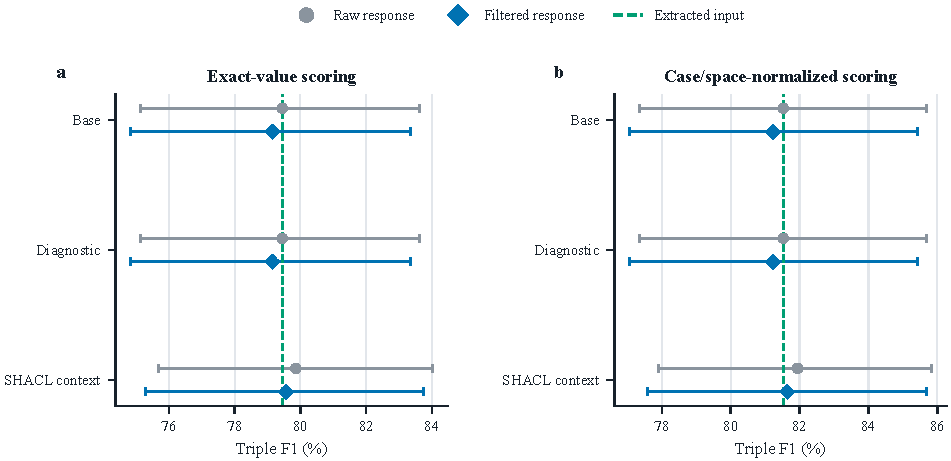
\includegraphics[width=0.98\textwidth]{figure/experiments/external_receipts.pdf}
\caption{首次收据评分。点表示平均 F1，误差线为 95\% 文档 bootstrap 置信区间。每个原始／过滤对照使用一个响应。虚线表示输入 F1。}
\label{fig:external_receipts}
\end{figure}
% End merged sections/external_receipts.tex

% Begin merged sections/reextraction_diagnostics.tex
\subsection{收据修复与重新抽取细节}
\label{app:reextraction_diagnostics}

我们在相同的 60 张新测试收据上再收集 240 个 Gemma 响应，比较有无索引下的修复与重新抽取。各设置共享来源行、字段含义、文档编号和输出上限；修复额外获得已有图。主分数差为过滤后的索引修复减索引重新抽取。全部 240 个响应的 JSON 都包含 Markdown 代码围栏。固定的严格解析器将其记为失败，各设置 F1 均为零。

采集后，我们去掉外层围栏，并执行相同模式检查。全部 240 个响应随即可解析。表~\ref{tab:reextraction_recovery}~给出这些补充评分。索引修复 F1 为 83.93\%，索引重新抽取为 61.05\%，配对差为 22.88 个百分点（95\% 置信区间：14.84 至 31.35）。

\begin{table}[t]
\centering
\caption{60 张收据在采集后的补充评分。围栏兼容处理去掉外层 Markdown 围栏。编号规范化还在过滤前分配已知文档编号。两者均使用保存的响应。}
\label{tab:reextraction_recovery}
\small
\begin{tabular}{lrrr}
\toprule
方法 & 围栏兼容 F1 & 编号规范化 F1 & 错误编号图数 \\
\midrule
重新抽取 & 0.6333 & 0.7256 & 18/60 \\
索引抽取 & 0.6105 & 0.7486 & 28/60 \\
修复率 & 0.7917 & 0.7917 & 0/60 \\
索引修复 & 0.8393 & 0.8393 & 0/60 \\
\bottomrule
\end{tabular}
\end{table}

索引重新抽取在 28 张图中给出错误文档编号；索引修复在全部 60 张图中使用正确编号。为四种设置统一分配已知编号后，索引重新抽取 F1 提高到 74.86\%，索引修复领先 9.07 个百分点（95\% 置信区间：5.22 至 13.10）。编号修正保持字段值不变。原来的 22.88 个百分点差距同时包含编号和字段值的影响。初始图构建成本与这些修复调用分别计算。

\paragraph{行索引覆盖的字段。}

我们在来源行中定位最初后续测试的 240 个参考字段。匹配保留大小写和标点，并清理空白。一个值跨越多行时，索引必须包含某次出现的全部行。240 个值中，188 个出现在索引行或邻近行，36 个出现在范围外，16 个与来源文本不同。对于覆盖的 188 个值，简单流程 精确返回 163 个，证据索引 返回 174 个。对于范围外的 36 个值，两者都返回 26 个；与来源不同的 16 个值，两者都未返回。索引净增加的十一项精确匹配来自覆盖组。

% Begin merged sections/call_policy_support.tex
\subsection{按可见错误调用修复}
\label{app:call_policy}

我们测试基于可见编号、关系、重复、字段数量和来源匹配错误的调用规则。它为每篇文档选择返回输入，或返回保存的修复输出。在 450 项模型构建与干净图混合流上，仅对 6.22\% 的输入调用修复，却漏掉 63.64\% 有参考差异的图。其 F1 为 94.46\%，始终调用修复为 95.82\%。可见检查漏掉许多缺失或字段分配错误的值。主方法对每篇文档都调用修复。

% Begin merged sections/offline_diagnostics.tex
\paragraph{早期选择器中的有用编辑。}

我们使用早期选择器保存的建议与试改图。这些运行早于表~\ref{tab:math_revision_selector}~中的共享特征和候选启动修改。对每篇文档，尝试模型编辑包的所有子集，并根据参考图为结果计分。执行保存编辑时关闭停止、成本和图边界检查。参考得分最高的子集称为 oracle。这项分析使用模型编辑包和参考值。

我们在 450 个输入上尝试 2,144 个子集，结果见表~\ref{tab:selection_bottlenecks}。注入缺陷输入中，86 张图未检测到违规，其中 72 张缺少参考字段，70 张存在能提高 F1 的建议子集。检查的试改中，212 项提高参考 F1，但效用分数不大于零。模型构建输入的对应数量为 8 张图和 1 项试改。

\begin{table}[t]
\centering
\caption{早期选择器结果，每组 225 个输入。oracle 利用参考答案寻找最佳保存子集。一篇文档可以有多次试改。}
\label{tab:selection_bottlenecks}
\small
\begin{tabular}{lrr}
\toprule
诊断项 & 受控输入 & 模型构建输入 \\
\midrule
预处理图 F1 & 0.8472 & 0.8799 \\
均匀选择器 F1 & 0.8472 & 0.8833 \\
固定建议 oracle F1 & 0.9964 & 0.9173 \\
初始未检出违规 & 86 & 198 \\
其中与参考不同的图 & 72 & 50 \\
其中存在可改善结果的图 & 70 & 8 \\
提高参考分数但效用非正的试改 & 212 & 1 \\
\bottomrule
\end{tabular}
\end{table}

去掉编辑成本使 67 篇注入缺陷文档的 F1 提高，158 篇不变，0 篇降低。模型构建输入中，0 篇提高，222 篇不变，3 篇降低。这三张图在清理后已经与参考不同。全部 148 个原本精确匹配的模型构建输入保留其 F1。注入缺陷输入的配对增益为 4.58 个百分点（95\% 文档 bootstrap 置信区间：3.69--5.54）。同一成本修改在两组输入上作用不同。


\subsection{图检查的时间与内存}
\label{sec:eval:scale}

我们在包含 1K--50K 条三元组的独立文档批次上，测量式~(\ref{eq:diagnostic_context})~中报告的耗时。完整扫描检查所有文档，局部更新只检查一篇已修改文档。完整扫描时间取七次运行的中位数，局部更新时间取 200 次运行的中位数，数值见表~\ref{tab:diagnostic_scaling}。内存统计构建批次时新增 Python 内存的峰值。源文本和模式对象共享，模型调用时间另计。

\begin{figure}[t]
\centering
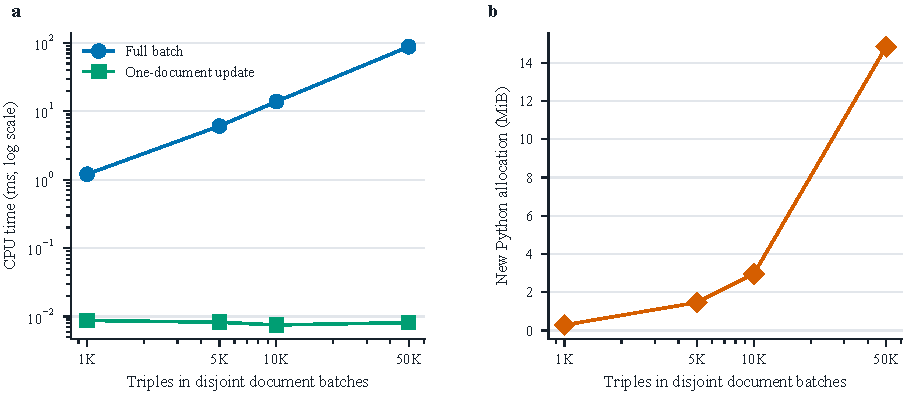
\includegraphics[width=0.98\textwidth]{figure/experiments/diagnostic_scaling.pdf}
\caption{独立文档批次的报告时间和内存。局部更新只检查一篇修改后的文档。内存统计共享源文本时新增的批次存储。}
\label{fig:diagnostic_scaling}
\end{figure}

\subsection{补充质量与抽取检查}
\label{sec:eval:external_benchmark}

Gemma 评判器在方法名称隐藏的条件下，为 180 个来源与三元组对打分。来源分数与精确参考有效性的 Pearson 相关系数为 $r=0.794$，Spearman 相关系数为 $\rho=0.807$（两者均有 $p<2.4\times10^{-40}$）。另外五次运行中，固定 50 项样本的均值都为 0.96。

我们在 45 篇均衡 TNEWS 文档上，将本文抽取器与 Neo4j Labs 的 \texttt{LLMGraphTransformer} 核心比较\citep{ref_neo4j_llm_graph_builder}。字段抽取器的类别准确率为 0.556，Graph Builder 为 0.533，配对检验为 $p=1.00$。

\subsection{请求成本与检查时间}
% Begin merged sections/audit_supporting.tex
\begin{table*}[t]
\centering
\caption{请求成本。平均时间包含重试和请求间隔等待。来源设置与排队时间另计。}
\label{tab:matched_cost}
\small
\resizebox{\textwidth}{!}{%
\begin{tabular}{llrrrr}
\toprule
输入 & 上下文 & 调用数 & 输入 token & 输出 token & 总耗时（秒） \\
\midrule
受控输入 & 基础提示 & 1.00 & 947 & 517 & 8.58 \\
受控输入 & 诊断提示 & 1.00 & 1017 & 512 & 8.61 \\
受控输入 & SHACL & 1.00 & 3080 & 513 & 8.45 \\
模型构建输入 & 基础提示 & 1.00 & 832 & 458 & 7.51 \\
模型构建输入 & 诊断提示 & 1.00 & 901 & 462 & 7.90 \\
模型构建输入 & SHACL & 1.00 & 2822 & 455 & 8.16 \\
\bottomrule
\end{tabular}%
}
\end{table*}
\begin{table*}[t]
\centering
\caption{图报告的时间和内存。内存统计新增批次存储峰值，单位为 MiB，源文本共享。}
\label{tab:diagnostic_scaling}
\small
\resizebox{\textwidth}{!}{%
\begin{tabular}{rrrrr}
\toprule
三元组 & 文档数 & 完整（毫秒） & 局部（毫秒） & 内存（MiB） \\
\midrule
1,000 & 143 & 1.20 & 0.009 & 0.29 \\
5,000 & 716 & 6.08 & 0.008 & 1.47 \\
10,000 & 1,434 & 13.90 & 0.008 & 2.96 \\
50,000 & 7,173 & 88.10 & 0.008 & 14.84 \\
\bottomrule
\end{tabular}%
}
\end{table*}
% End merged sections/audit_supporting.tex

\clearpage
\section*{译文附页：图中文字对照}

本页对照原图中的英文标注。图形、数据点、颜色和数值沿用英文论文。方法名称在正文和表格中采用以下中文写法。

\begin{center}
\small
\begin{tabularx}{\textwidth}{lX}
\toprule
原图方法名 & 中文名称 \\
\midrule
Source-field Copy & 来源字段复制 \\
No Repair & 不修复 \\
Rule Only & 仅规则 \\
SHACL-style & SHACL 风格修复 \\
Direct LLM & 直接调用模型 \\
ReAct-style & ReAct 风格智能体 \\
Simple Pipeline / Simple & 简单流程 \\
Diagnosis + Gate & 诊断＋门控 \\
Evidence Index / Index & 证据索引 \\
Base & 基础提示 \\
Diagnostic & 诊断提示 \\
SHACL context & SHACL 上下文 \\
\bottomrule
\end{tabularx}
\end{center}

\paragraph{图~\ref{fig:scale_relationship}：三个检查范围。}
\begin{itemize}
\item 输入：One document · three views 为“一篇文档、三个视角”；Source $X$ 为“原文 $X$”；Task schema 为“任务模式”；Head 为“头节点”；Relations 为“关系”。示例 Merchant: ALPHA、Total: 42.00 表示“商户：ALPHA、总额：42.00”。
\item Local scope 为“局部范围”；Incidence + duplicates 为“节点连接与重复”；merchant 为“商户”；isolated node 为“孤立节点”；Repeated fact → duplicate flag 为“事实重复，标记为重复”；No incident edge → local flag 为“没有关联边，标记为局部问题”；Scores: incidence, uniqueness 为“分数：节点连接、唯一性”。
\item Graph scope 为“图范围”；Head + relation schema 为“头节点与关系模式”；seller 为“卖方”；seller is not permitted 为“seller 关系不在允许名单内”；$H(t)$ 的说明为“头节点匹配 d1”；$R(t)$ 的说明为“关系被允许”；Score: rule consistency 为“分数：规则一致性”。
\item Source scope 为“来源范围”；Value ↔ source text 为“值与源文本对应”；Source excerpt 为“来源片段”；Graph value: 49.00 → absent 为“图中取值 49.00 在原文中不存在”；$S(t;X)$ 的说明为“非空值出现在原文中”；Score: source support 为“分数：来源支持”。底部 Shared report 表示“共享报告：重复计数、失败检查、已出现的关系”。
\end{itemize}

\paragraph{图~\ref{fig:framework_overview}：路由与编辑选择。}
\begin{itemize}
\item Input graph 为“输入图”；Document graph $G_t$ 为“文档图 $G_t$”；Source $X$ 为“原文 $X$”。示例 merchant、total 分别为“商户、总额”，图中的 49.00 对应来源中的 42.00。
\item Quality profile 为“质量评估概况”；Four quality scores 为“四项质量分数”：Incidence、Uniqueness、Rule consistency、Source support，分别为“节点连接、唯一性、规则一致性、来源支持”。Four graph statistics 为“四项图统计量”：Nodes、triples、Density、violations，即“节点数、三元组数、密度、违规数”。
\item Neural routing 为“神经路由”；8 inputs → router 为“八个输入进入路由器”；Repair trigger 为“修复触发分数”；Scope prior $\pi$ 为“范围先验 $\pi$”；Local、Graph、Source 为“局部、图、来源”。Hard flags or candidates override a low trigger 表示“存在硬规则标记或候选时，较低触发分数仍会启动试改”。
\item Edit selection 为“编辑选择”；Candidate edits 为“候选编辑”；Fixed model bundles + rule-derived proposals 为“固定模型编辑包加规则建议”；Delete、Retype、Add 分别为“删除、改关系、添加”。Trial graphs 为“试改图”；Bounds + utility $U(a)$ 为“边界与效用 $U(a)$”。选择步骤为“选择可执行且 $U(a)>0$ 最高的一项编辑”。
\item Commit one edit → $G_{t+1}$ 为“执行一项编辑，得到 $G_{t+1}$”；随后“保留决策日志，重新评估接受后的图”。底部说明：顺序变体在每次接受编辑后重新评估；没有可执行的正效用编辑时停止。
\end{itemize}

\paragraph{图~\ref{fig:optimization_flow}：一次试改循环。}
\begin{itemize}
\item Route 为“路由”：当前图 $G_t$ 输入四项评估分数和四项图统计量。Learned router 为“学习得到的路由器”；输出修复分数 $p(\mathrm{repair})$ 和范围先验 $\pi$。存在硬规则违规或已提供候选时，低触发分数仍继续试改。
\item Propose 为“提出候选”：Model proposals 为“模型建议”；Fixed edit bundles grouped by relation 为“按关系分组的固定编辑包”；Rule proposals 为“规则建议”；Detected violations + explicit source fields 为“检测到的违规与明确来源字段”。动作是删除、改关系和添加；Deduplicate candidates 为“对候选去重”。
\item Evaluate trials 为“评估试改”：在 $G_t$ 的独立副本上分别尝试 $a_1,a_2,a_3$，得到试改图。Recompute profile and flags 为“重新计算评估概况与标记”；Check bounds; calculate $U(a)$ 为“检查边界，计算 $U(a)$”。
\item Select 为“选择”：先判断是否允许执行、是否满足 $U(a)>0$，再在合格编辑中选择最高效用，执行一项编辑，使 $G_t$ 变为 $G_{t+1}$。
\item Utility $U(a)$ 的文字说明为“质量增益＋硬规则违规减少－编辑成本＋对数范围先验＋建议置信度”。Trial-state constraints 为“试改状态约束”，包括“恢复边界、单项分数有限回退、密度上界、非空图保护”。
\item 底部说明：重新评估执行后的图，并在 12 步范围内重复；没有合格编辑或达到 12 步时停止。提前退出条件为“没有已提供候选，且低触发分数下没有硬规则标记，或没有检测到违规”。
\end{itemize}

\paragraph{图~\ref{fig:repair_benchmark_results}：受控修复。}
a 中 Quality with 95\% bootstrap intervals 为“质量分数及 95\% bootstrap 区间”；Defect repair、Triple F1、Exact graph 为“缺陷修复、三元组 F1、整图匹配”；Held-out score 为“预留测试得分”。b 中 Quality--latency trade-off 为“质量与耗时的权衡”；纵轴为“缺陷修复率”，横轴为“每篇文档耗时（秒）”。圆形和方形表示一次调用，菱形表示两次调用。方法名见本附页开头。

\paragraph{图~\ref{fig:natural_stratified}：按输入类型分组。}
Extracted input 为“抽取输入”；Simple pipeline 为“简单流程”；All inputs 为“全部输入”；Valid JSON 为“有效 JSON”；Imperfect valid JSON 为“有效但与参考不同的 JSON”；Malformed JSON 为“无效 JSON”。$n$ 表示该组样本数。a 的横轴为“三元组 F1（\%）”，b 为“整图精确匹配（\%）”。其他方法名见本附页开头。

\paragraph{图~\ref{fig:matched_mechanisms}：机制对照。}
Raw candidate 为“原始候选”；Gated pipeline 为“门控过滤流程”；Sequential optimizer 为“顺序选择器”。a 为“受控输入”，b 为“模型构建输入”，c 为“保存的候选”；Archived candidates 表示“历史保存候选”。三幅图横轴均为“三元组 F1（\%）”。Base、Diagnostic、SHACL context 的对应中文见开头。

\paragraph{图~\ref{fig:receipt_followup}：新收据。}
Extracted input 为“抽取输入”，a 的横轴为“三元组 F1（\%）”。b 的三项为“简单流程减输入”“索引减简单流程”“索引减 SHACL”，横轴 Paired F1 difference (points) 为“配对 F1 差（百分点）”。方法名见开头。

\paragraph{图~\ref{fig:recovery_ablation}：析因与来源行。}
a 的 Factorial main effects 为“析因主效应”；Preprocessing、Diagnosis、Gate 分别为“预处理、诊断、门控”；Controlled、Natural 分别为“受控输入、模型构建输入”。b 的 Receipt context contrasts 为“收据上下文对照”；Full、Random、Anchors 分别为“完整索引、随机索引、仅锚点”；No-def. full 为“无字段定义的完整索引”，No-def. simple 为“无字段定义的简单流程”。各项依次比较“完整减简单”“完整减随机”“完整减锚点”“完整减无定义完整”“简单减无定义简单”。横轴均为“配对 F1 变化（百分点）”。

\paragraph{图~\ref{fig:cuad}：合同。}
Initial extraction、Simple repair、Indexed repair、Indexed re-extraction 分别为“初始抽取、简单流程修复、索引修复、索引重新抽取”。横轴 Document mean F1 (\%) with 95\% bootstrap interval 为“文档平均 F1（\%）及 95\% bootstrap 区间”。

\paragraph{图~\ref{fig:external_receipts}：首次收据。}
Raw response、Filtered response、Extracted input 分别为“原始响应、过滤后响应、抽取输入”。a 的 Exact-value scoring 为“精确值评分”，b 的 Case/space-normalized scoring 为“大小写与空白规范化评分”。横轴为“三元组 F1（\%）”。提示名称见本附页开头。

\paragraph{图~\ref{fig:diagnostic_scaling}：检查规模。}
Full batch 为“完整批次”；One-document update 为“单文档更新”。a 的纵轴 CPU time (ms; log scale) 为“CPU 时间（毫秒，对数坐标）”。b 的纵轴 New Python allocation (MiB) 为“新增 Python 内存分配（MiB）”。两幅图横轴 Triples in disjoint document batches 为“互相独立的文档批次中的三元组数”，1K、5K、10K、50K 分别表示一千、五千、一万和五万条。


\end{document}
